\documentclass[a4paper,11pt]{article}
\pdfoutput=1 % if your are submitting a pdflatex (i.e. if you have
             % images in pdf, png or jpg format)

\usepackage{jinstpub} % for details on the use of the package, please
                     % see the JINST-author-manual
\usepackage{lineno}
\usepackage{amsmath}

\linenumbers
\hyphenation{MicroBooNE}
%\linespread{2} %temp double spacing for style reviewers

%\author{The MicroBooNE Collaboration}


% Authors in alphabetical order
\author[g]{R.~Acciarri}
\author[bb]{C.~Adams}
\author[h]{R.~An}
\author[c]{J.~Anthony}
\author[y]{J.~Asaadi}
\author[a]{M.~Auger}
\author[g]{L.~Bagby}
\author[bb]{S.~Balasubramanian}
\author[g]{B.~Baller}
\author[n]{C.~Barnes}
\author[q]{G.~Barr}
\author[q]{M.~Bass}
\author[z]{F.~Bay}
\author[b]{M.~Bishai}
\author[j]{A.~Blake}
\author[i]{T.~Bolton}
\author[m]{L.~Bugel}
\author[f]{L.~Camilleri}
\author[f]{D.~Caratelli}
\author[g]{B.~Carls}
\author[g]{R.~Castillo~Fernandez}
\author[g]{F.~Cavanna}
\author[b]{H.~Chen}
\author[r]{E.~Church}
\author[l,f]{D.~Cianci}
\author[w]{E.~Cohen}
\author[m]{G.~H.~Collin}
\author[m]{J.~M.~Conrad}
\author[u]{M.~Convery}
\author[f]{J.~I.~Crespo-Anad\'{o}n}
\author[q]{M.~Del~Tutto}
\author[j]{D.~Devitt}
\author[s]{S.~Dytman}
\author[u]{B.~Eberly}
\author[a]{A.~Ereditato}
\author[c]{L.~Escudero Sanchez}
\author[v]{J.~Esquivel}
\author[bb]{B.~T.~Fleming}
\author[d]{W.~Foreman}
\author[l]{A.~P.~Furmanski}
\author[l]{D.~Garcia-Gamez}
\author[k]{G.~T.~Garvey}
\author[f]{V.~Genty}
\author[a]{D.~Goeldi}
\author[i,x]{S.~Gollapinni}
\author[s]{N.~Graf}
\author[bb]{E.~Gramellini}
\author[g]{H.~Greenlee}
\author[e]{R.~Grosso}
\author[q]{R.~Guenette}
\author[bb]{A.~Hackenburg}
\author[v]{P.~Hamilton}
\author[m]{O.~Hen}
\author[l]{J.~Hewes}
\author[l]{C.~Hill}
\author[d]{J.~Ho}
\author[i]{G.~Horton-Smith}
\author[k]{E.-C.~Huang}
\author[g]{C.~James}
\author[c]{J.~Jan~de~Vries}
\author[aa]{C.-M.~Jen}
\author[s]{L.~Jiang}
\author[e]{R.~A.~Johnson}
\author[b]{J.~Joshi}
\author[g]{H.~Jostlein}
\author[f]{D.~Kaleko}
\author[l,f]{G.~Karagiorgi}
\author[g]{W.~Ketchum}
\author[b]{B.~Kirby}
\author[g]{M.~Kirby}
\author[g]{T.~Kobilarcik}
\author[a]{I.~Kreslo}
\author[q]{A.~Laube}
\author[b]{Y.~Li}
\author[j]{A.~Lister}
\author[h]{B.~R.~Littlejohn}
\author[g]{S.~Lockwitz}
\author[a]{D.~Lorca}
\author[k]{W.~C.~Louis}
\author[a]{M.~Luethi}
\author[g]{B.~Lundberg}
\author[bb]{X.~Luo}
\author[g]{A.~Marchionni}
\author[aa]{C.~Mariani}
\author[c]{J.~Marshall}
\author[h]{D.~A.~Martinez~Caicedo}
\author[i]{V.~Meddage}
\author[o]{T.~Miceli}
\author[k]{G.~B.~Mills}
\author[m]{J.~Moon}
\author[b]{M.~Mooney}
\author[g]{C.~D.~Moore}
\author[n]{J.~Mousseau}
\author[l]{R.~Murrells}
\author[s]{D.~Naples}
\author[t]{P.~Nienaber}
\author[j]{J.~Nowak}
\author[g]{O.~Palamara}
\author[s]{V.~Paolone}
\author[o]{V.~Papavassiliou}
\author[o]{S.~F.~Pate}
\author[g]{Z.~Pavlovic}
\author[w]{E.~Piasetzky}
\author[l]{D.~Porzio}
\author[v]{G.~Pulliam}
\author[b]{X.~Qian}
\author[g]{J.~L.~Raaf}
\author[i]{A.~Rafique}
\author[u]{L.~Rochester}
\author[a]{C.~Rudolf~von~Rohr}
\author[bb]{B.~Russell}
\author[d]{D.~W.~Schmitz}
\author[g]{A.~Schukraft}
\author[f]{W.~Seligman}
\author[f]{M.~H.~Shaevitz}
\author[a]{J.~Sinclair}
\author[g]{E.~L.~Snider}
\author[v]{M.~Soderberg}
\author[l]{S.~S{\"o}ldner-Rembold}
\author[q]{S.~R.~Soleti}
\author[g]{P.~Spentzouris}
\author[n]{J.~Spitz}
\author[e]{J.~St.~John}
\author[g]{T.~Strauss}
\author[l]{A.~M.~Szelc}
\author[p]{N.~Tagg}
\author[f]{K.~Terao}
\author[c]{M.~Thomson}
\author[g]{M.~Toups}
\author[u]{Y.-T.~Tsai}
\author[bb]{S.~Tufanli}
\author[u]{T.~Usher}
\author[k]{R.~G.~Van~de~Water}
\author[b]{B.~Viren}
\author[a]{M.~Weber}
\author[s]{D.~A.~Wickremasinghe}
\author[g]{S.~Wolbers}
\author[m]{T.~Wongjirad}
\author[o]{K.~Woodruff}
\author[g]{T.~Yang}
\author[m]{L.~Yates}
\author[g]{G.~P.~Zeller}
\author[d]{J.~Zennamo}
\author[b]{C.~Zhang}

% Institutions in alphabetical order
\affiliation[a]{Universit{\"a}t Bern, Bern CH-3012, Switzerland}
\affiliation[b]{Brookhaven National Laboratory (BNL), Upton, NY, 11973, USA}
\affiliation[c]{University of Cambridge, Cambridge CB3 0HE, United Kingdom}
\affiliation[d]{University of Chicago, Chicago, IL, 60637, USA}
\affiliation[e]{University of Cincinnati, Cincinnati, OH, 45221, USA}
\affiliation[f]{Columbia University, New York, NY, 10027, USA}
\affiliation[g]{Fermi National Accelerator Laboratory (FNAL), Batavia, IL 60510, USA}
\affiliation[h]{Illinois Institute of Technology (IIT), Chicago, IL 60616, USA}
\affiliation[i]{Kansas State University (KSU), Manhattan, KS, 66506, USA}
\affiliation[j]{Lancaster University, Lancaster LA1 4YW, United Kingdom}
\affiliation[k]{Los Alamos National Laboratory (LANL), Los Alamos, NM, 87545, USA}
\affiliation[l]{The University of Manchester, Manchester M13 9PL, United Kingdom}
\affiliation[m]{Massachusetts Institute of Technology (MIT), Cambridge, MA, 02139, USA}
\affiliation[n]{University of Michigan, Ann Arbor, MI, 48109, USA}
\affiliation[o]{New Mexico State University (NMSU), Las Cruces, NM, 88003, USA}
\affiliation[p]{Otterbein University, Westerville, OH, 43081, USA}
\affiliation[q]{University of Oxford, Oxford OX1 3RH, United Kingdom}
\affiliation[r]{Pacific Northwest National Laboratory (PNNL), Richland, WA, 99352, USA}
\affiliation[s]{University of Pittsburgh, Pittsburgh, PA, 15260, USA}
\affiliation[t]{Saint Mary's University of Minnesota, Winona, MN, 55987, USA}
\affiliation[u]{SLAC National Accelerator Laboratory, Menlo Park, CA, 94025, USA}
\affiliation[v]{Syracuse University, Syracuse, NY, 13244, USA}
\affiliation[w]{Tel Aviv University, Tel Aviv, Israel, 69978}
\affiliation[x]{University of Tennessee, Knoxville, TN, 37996, USA}
\affiliation[y]{University of Texas, Arlington, TX, 76019, USA}
\affiliation[z]{TUBITAK Space Technologies Research Institute, METU Campus, TR-06800, Ankara, Turkey}
\affiliation[aa]{Center for Neutrino Physics, Virginia Tech, Blacksburg, VA, 24061, USA}
\affiliation[bb]{Yale University, New Haven, CT, 06520, USA}





% \title{Improved Neutrino-Induced-Muon Momentum Determination by Multiple Coulomb Scattering in the MicroBooNE LArTPC from Tuning the Highland Formula}
\title{Determination of muon momentum in the MicroBooNE LArTPC using an improved model of multiple Coulomb scattering}


%% %simple case: 2 authors, same institution
%% \author{A. Uthor}
%% \author{and A. Nother Author}
%% \affiliation{Institution,\\Address, Country}

% % more complex case: 4 authors, 3 institutions, 2 footnotes
% \author[a,b,1]{F. Irst,\note{Corresponding author.}}
% \author[c]{S. Econd,}
% \author[a,2]{T. Hird\note{Also at Some University.}}
% \author[c,2]{and Fourth}

% % The "\note" macro will give a warning: "Ignoring empty anchor..."
% % you can safely ignore it.

% \affiliation[a]{One University,\\some-street, Country}
% \affiliation[b]{Another University,\\different-address, Country}
% \affiliation[c]{A School for Advanced Studies,\\some-location, Country}

% % e-mail addresses: only for the forresponding author
% \emailAdd{first@one.univ}


\abstract{%Liquid argon time projection chambers (LArTPCs) are an important detector technology for neutrino physics. This technology provides precise three-dimensional reconstruction of charged particle tracks that traverse the detector medium. 
%The MicroBooNE experiment is a LArTPC at the Fermi National Accelerator laboratory with active volume dimensions of 2.6 m width $\times$ 2.3 m height $\times$ 10.4 m length located in the Booster Neutrino Beamline (BNB) which has a peak neutrino energy of about 0.7 GeV. 
We discuss a technique for measuring a charged particle's momentum by means of multiple Coulomb scattering (MCS) in the MicroBooNE liquid argon time projection chamber (LArTPC). This method does not require the full particle ionization track to be contained inside of the detector volume as other track momentum reconstruction methods do (range-based momentum reconstruction and calorimetric momentum reconstruction). We motivate use of this technique, describe a tuning of the underlying phenomenological formula, quantify its performance on fully contained beam-neutrino-induced muon tracks both in simulation and in data, and quantify its performance on exiting muon tracks in simulation. We find agreement between data and simulation for contained tracks, with a small bias in the momentum reconstruction and with resolutions that vary as a function of track length, improving from about 10\% for the shortest (one meter long) tracks to 5\% for longer (several meter) tracks. For simulated exiting muons with at least one meter of track contained, we find a similarly small bias, and a resolution which is less than 15\% for muons with momentum below 2 GeV/c though higher at higher momenta.}


% \keywords{Only keywords from JINST's keywords list please}


% \arxivnumber{1234.56789} % only if you have one


% \collaboration{\includegraphics[height=17mm]{example-image}\\[6pt]
%   XXX collaboration}
% or
% \collaboration[c]{on behalf of XXX collaboration}


% if you write for a special issue this may be useful
% \proceeding{N$^{\text{th}}$ Workshop on X\\
%   when\\
%   where}



\begin{document}
\maketitle
\flushbottom

\section{Introduction and motivation}\label{sec:intro}

In this paper we summarize the theory of multiple Coulomb scattering (MCS) and describe how the underlying Highland formula is retuned based on Monte Carlo simulation for use in liquid-argon time-projection chambers (LArTPCs). We present a maximum likelihood based algorithm that is used to determine the momentum of particles in a LArTPC. The only way to determine the momentum of a particle that exits the active volume of a LArTPC is through MCS measurements. We demonstrate that this technique works well for a sample of fully contained muons from Booster Neutrino Beam (BNB) $\nu_\mu$ charged-current (CC) interactions, and determine the resolutions and biases of the measurement. In addition we demonstrate the performance of the method on simulated exiting tracks.\\

MicroBooNE (Micro Booster Neutrino Experiment) is an experiment that uses a large LArTPC to investigate the excess of low energy events observed by the MiniBooNE experiment \cite{Aguilar-Arevalo:2013pmq} and to study neutrino-argon cross-sections. MicroBooNE is the first detector of the Short-Baseline Neutrino (SBN) \cite{SBNwhitepaper} physics program at the Fermi National Accelerator Laboratory (Fermilab), to be joined by two other LArTPCs: the Short Baseline Near Detector (SBND) and the Imaging Cosmic And Rare Underground Signal (ICARUS) detector \cite{ICARUS_maincitation}. In addition to producing valuable physics output, MicroBooNE serves as an important source of detector and reconstruction development for future LArTPC experiments, such as the Deep Underground Neutrino Experiment (DUNE) \cite{DUNE_citation}.\\%MicroBooNE also performs important research and development in terms of detector technology and event reconstruction techniques for future LArTPC experiments including DUNE (Deep Underground Neutrino Experiment) \cite{DUNE_citation}.\\



The MicroBooNE detector \cite{ub_detectorpaper} consists of a rectangular time-projection chamber (TPC) with dimensions 2.6 m $\times$ 2.3 m $\times$ 10.4 m (width $\times$ height $\times$ length) located 470 m downstream from the Booster Neutrino Beam (BNB) target \cite{BNB_citation}. LArTPCs allow for precise three-dimensional reconstruction of particle interactions. For later reference, the $z$ axis of the detector is horizontal, along the direction of the BNB, while the $x$ direction of the TPC corresponds to the drift coordinate and the $y$ direction is the vertical direction. The mass of active liquid argon contained within the MicroBooNE TPC volume is 89 tons, out of a total mass of 170 tons.\\

A set of 32 photomultiplier tubes (PMTs) and three planes of wires with 3 mm spacing at angles of 0, and $\pm$ 60 degrees with respect to the vertical are located in the TPC for event reconstruction. The cathode plane operating voltage is -70 kV. As illustrated in figure \ref{detector_fig}, a neutrino in the beam interacts with an argon nucleus and the charged outgoing particles traverse the medium, lose energy and leave an ionization trail. The resulting ionization electrons drift in a 273 $\text{V/cm}$ electric field to the wire planes constituting the anode. The passage of these electrons through the first two wire planes induces a signal in the wires, and their collection on the third plane also generates a signal. These signals are used to create three distinct two-dimensional views (in terms of wire and time) of the event. Combining these wire signals allow for full three-dimensional reconstruction of the event, with PMT signals providing information about the absolute drift ($x$) coordinate. The boundaries of the fiducial volume used in this analysis are set back from the six faces of the active volume by distances of between 20 and 37 cm, depending on the face, to reduce the impact of electric-field non-uniformities near the edges of the TPC. This volume corresponds to a mass of 55 tons.\\

\begin{figure}[ht!]
\centering
	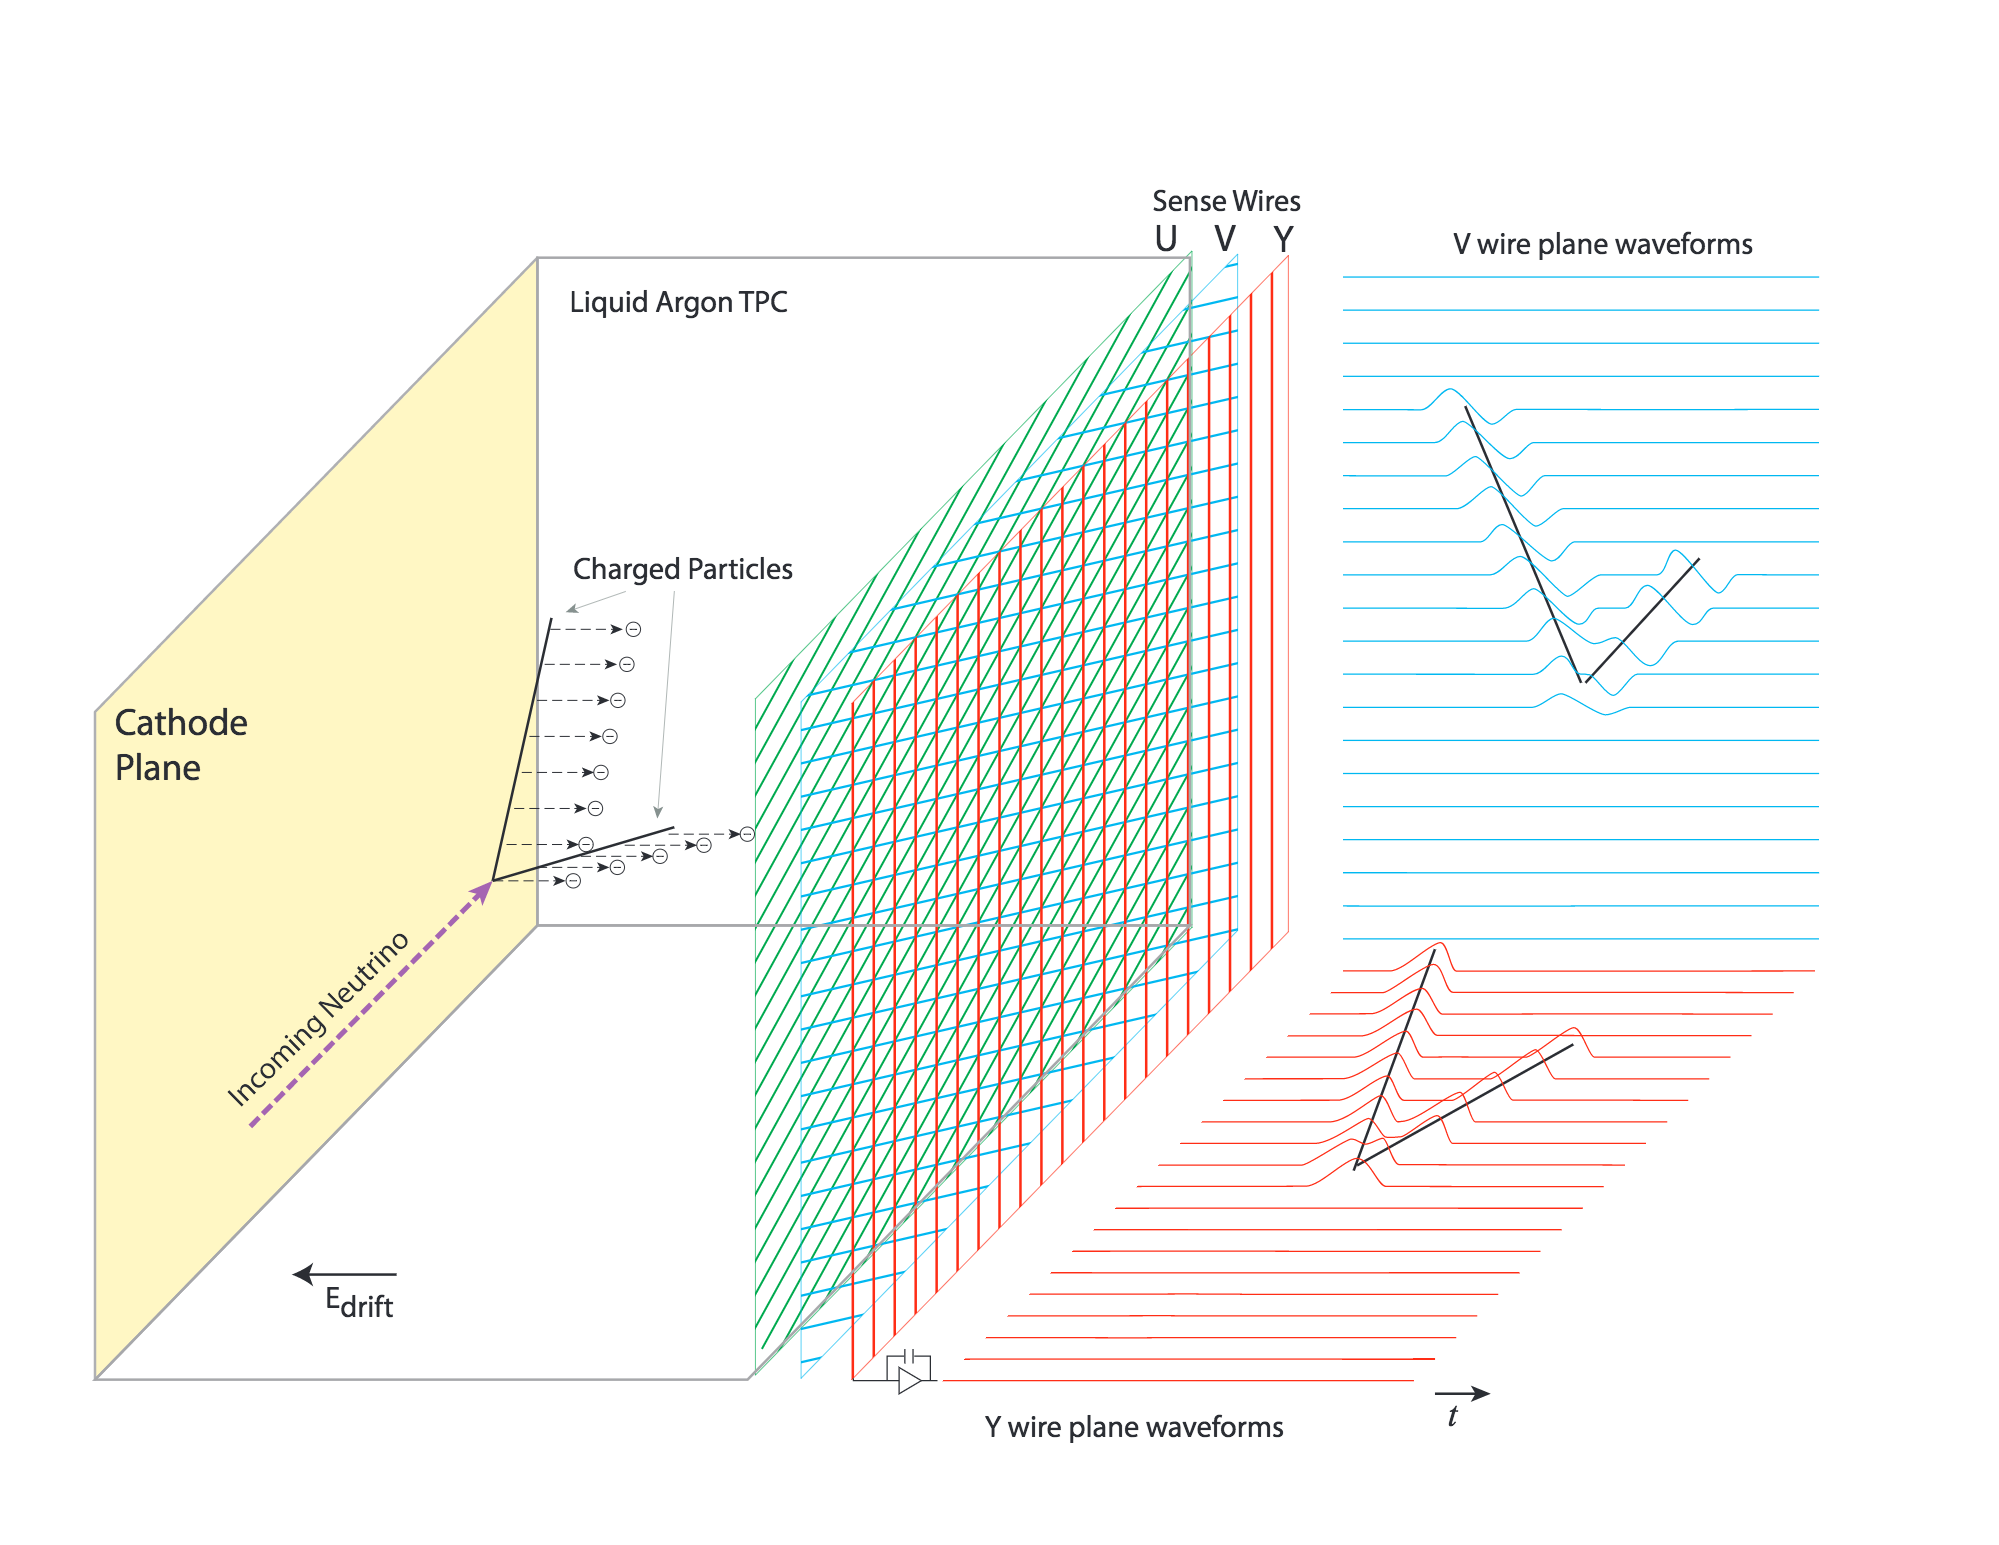
\includegraphics[width=0.9\textwidth]{Figures/static_figs/detector2.png} \\
\caption{A diagram of the time projection chamber of the MicroBooNE detector \cite{ub_detectorpaper}. PMTs (not shown) are located behind the wire planes.}\label{detector_fig}
\end{figure}

The Booster Neutrino Beam (BNB) is composed predominantly of muon neutrinos ($\nu_\mu$) with a peak neutrino energy of about 0.7 GeV. Some of these neutrinos undergo charge-current ($\nu_\mu$CC) interactions in the TPC and produce muons and other particles. For muon tracks that are completely contained in the TPC, we calculate the momentum with a measurement of the length of the particle's track, or with calorimetric measurements which come from wire signal size measurements. Around half of the muons from BNB $\nu_\mu$CC interactions in MicroBooNE are not fully contained in the TPC, and therefore using an established length-based or calorimetry-based method to determine the momenta for these uncontained tracks is not a possibility; the only way to determine their momenta is through MCS. \\

\section{Multiple Coulomb scattering}

Multiple Coulomb scattering occurs when a charged particle traverses a medium and undergoes electromagnetic scattering off atomic nuclei. This scattering perturbs the original trajectory of the particle within the material (figure \ref{mcs_nocap_fig}). For a given initial momentum $p$, the angular deflection scatters of a particle in either the $x'$ direction or $y'$ direction (as indicated in the aforementioned figure) form a Gaussian distribution centered at zero with an RMS width, $\sigma_o^{\text{HL}}$, given by the Highland formula \cite{highland}\cite{highland-lynch-dahl} 

\begin{equation}\label{highland_eqtn}
	\sigma_o^{\text{HL}}=\frac{S_2}{p\beta c}z\sqrt{\frac{\ell}{X_0}}\left[1+\epsilon\times\ln\left(\frac{\ell}{X_0}\right)\right],
\end{equation}

\noindent where $\beta$ is the ratio of the particle's velocity to the speed of light (assuming the particle is a muon), $\ell$ is the distance traveled inside the material, $z$ is the magnitude of the charge of the particle (unity, for the case of muons), and $X_0$ is the radiation length of the target material (taken to be a constant $14$~cm in liquid argon). $S_2$ and $\epsilon$ are parameters determined to be 13.6 MeV and 0.0038, respectively. In this study, a modified version of the Highland formula is used that includes a detector-inherent angular resolution term, $\sigma_o^{\text{res}}$
\begin{equation}\label{modified_highland_eqtn}
\sigma_{o} = \sqrt{ (\sigma_o^{\text{HL}})^2 + (\sigma_o^{\text{res}})^2}.% = \sqrt{ (\frac{13.6\  \text{MeV}}{p\beta c}z\sqrt{\frac{\ell}{X_0}}\Big[1+0.0038\text{ln}\Big(\frac{\ell}{X_0}\Big)\Big])^2 + (\sigma_o^{res})^2 }
\end{equation}
For this analysis, the $\sigma_o^{\text{res}}$ term is given a fixed value of 3 mrad which has been determined to be an acceptable value based on MicroBooNE simulation studies of muons at higher momenta. At 4.5 GeV/c muon momentum and $l\approx X_0$, equation \ref{highland_eqtn} predicts an RMS angular scatter of 3 mrad, comparable to the detector resolution. The fully contained muons addressed in this analysis have momenta below $1.5$~$\text{GeV/c}$, making the impact of this detector resolution minimal for that sample.\\

With the Highland formula, the momentum of a track-like particle can be determined using only the 3D reconstructed track information, without any calorimetric or track range information. In neutrino physics experiments, emulsion detectors like the DONUT \cite{DONUT_paper} and OPERA \cite{OPERA_paper} Collaborations have used MCS to determine particle momenta. Additionally, the MACRO \cite{MACRO_paper} Collaboration at Gran Sasso Laboratory utilized this technique. For LArTPCs, the ICARUS Collaboration has described MCS-based determination of particle momentum using a variety of methods \cite{icarus_mcs_paper,new_icarus_paper}. The likelihood-based method, discussed in this paper for use in the MicrobooNE detector and described in detail in section \ref{MCS_technique_section}, has improved on the ICARUS method by tuning the underlying phenomenological formula.


\begin{figure}[ht!]
\centering
	\includegraphics[width=0.9\textwidth]{Figures/static_figs/mcs_nocap_highres.pdf} \\
\caption{The particle's trajectory is deflected as it traverses the material. The angular scatter in the labeled $x'$ plane is shown as $\theta_x$.}\label{mcs_nocap_fig}
\end{figure}












\subsection{Tuning the Highland formula for argon}\label{highland_tuning_section}

The Highland formula as written in equation \ref{highland_eqtn} originates from a 1991 publication by G. R. Lynch and O. I. Dahl \cite{highland-lynch-dahl}. The parameters in the equation ($S_2$ and $\epsilon$) were determined using a global fit over MCS simulated data using a modified GEANT simulation package of 14 different elements and 7 thickness ranges. All of the simulated particles were relativistic, with $\beta=1$. The materials studied ranged from hydrogen (with Z=1) to uranium (with Z=92). Given that the parameters in the formula were determined from a single fit to a wide range of Z with a wide range of material thicknesses, there is reason to believe that these parameters should differ for scattering specifically in liquid argon with $l \approx X_0$. There is also reason to believe that these parameters might be momentum-dependent for particles with $\beta < 1$, which is the case for some of the contained muons in this analysis.\\

In order to re-tune these parameters to liquid argon, a large sample of muons are simulated with GEANT4\footnote{The GEANT4 version used in this simulation is 4.9.6.} \cite{GEANT4_citation} in the MicroBooNE TPC and their true angular scatters are used in a fit, with $l = X_0$. The reason for using $l = X_0$ is that the Highland formula simplifies to remove its dependence on $\epsilon$

\begin{equation}\label{highland_simplified}
	\sigma_o^{\text{HL}}=\frac{S_2}{p\beta c}.
\end{equation}

The $S_2$ parameter in equation \ref{highland_simplified} is fit for as a function of true muon momentum at each scatter, in order to explore the $\beta$ dependence of this parameter. The fitted parameter value as a function of true momentum is shown in figure \ref{retune_highland_fig1}.


 % was used to compute the RMS scattering angles along these tracks, using the true momentum of the muon at the start of each segment. The $13.6$ constant in this equation was varied such that a histogram of angular scatters divided by $\sigma_o$ was Gaussian with a width of unity\footnote{Note that Lynch and Dahl recommend fitting only the central portion (E.G. 98\%) of this distribution to mitigate the effect of large angle (non-Gaussian) scatters which are not well described by the Highland formula, but in this analysis the entire distribution is fit as the entire distribution is what is used in the algorithm itself. Fitting to the central 98\% was found to have little effect on the result of this analysis.}. To explore the potential $\beta$ dependence, this fitting was done in bins of true segment momentum. .\\

\begin{figure}[ht!]
\begin{center}
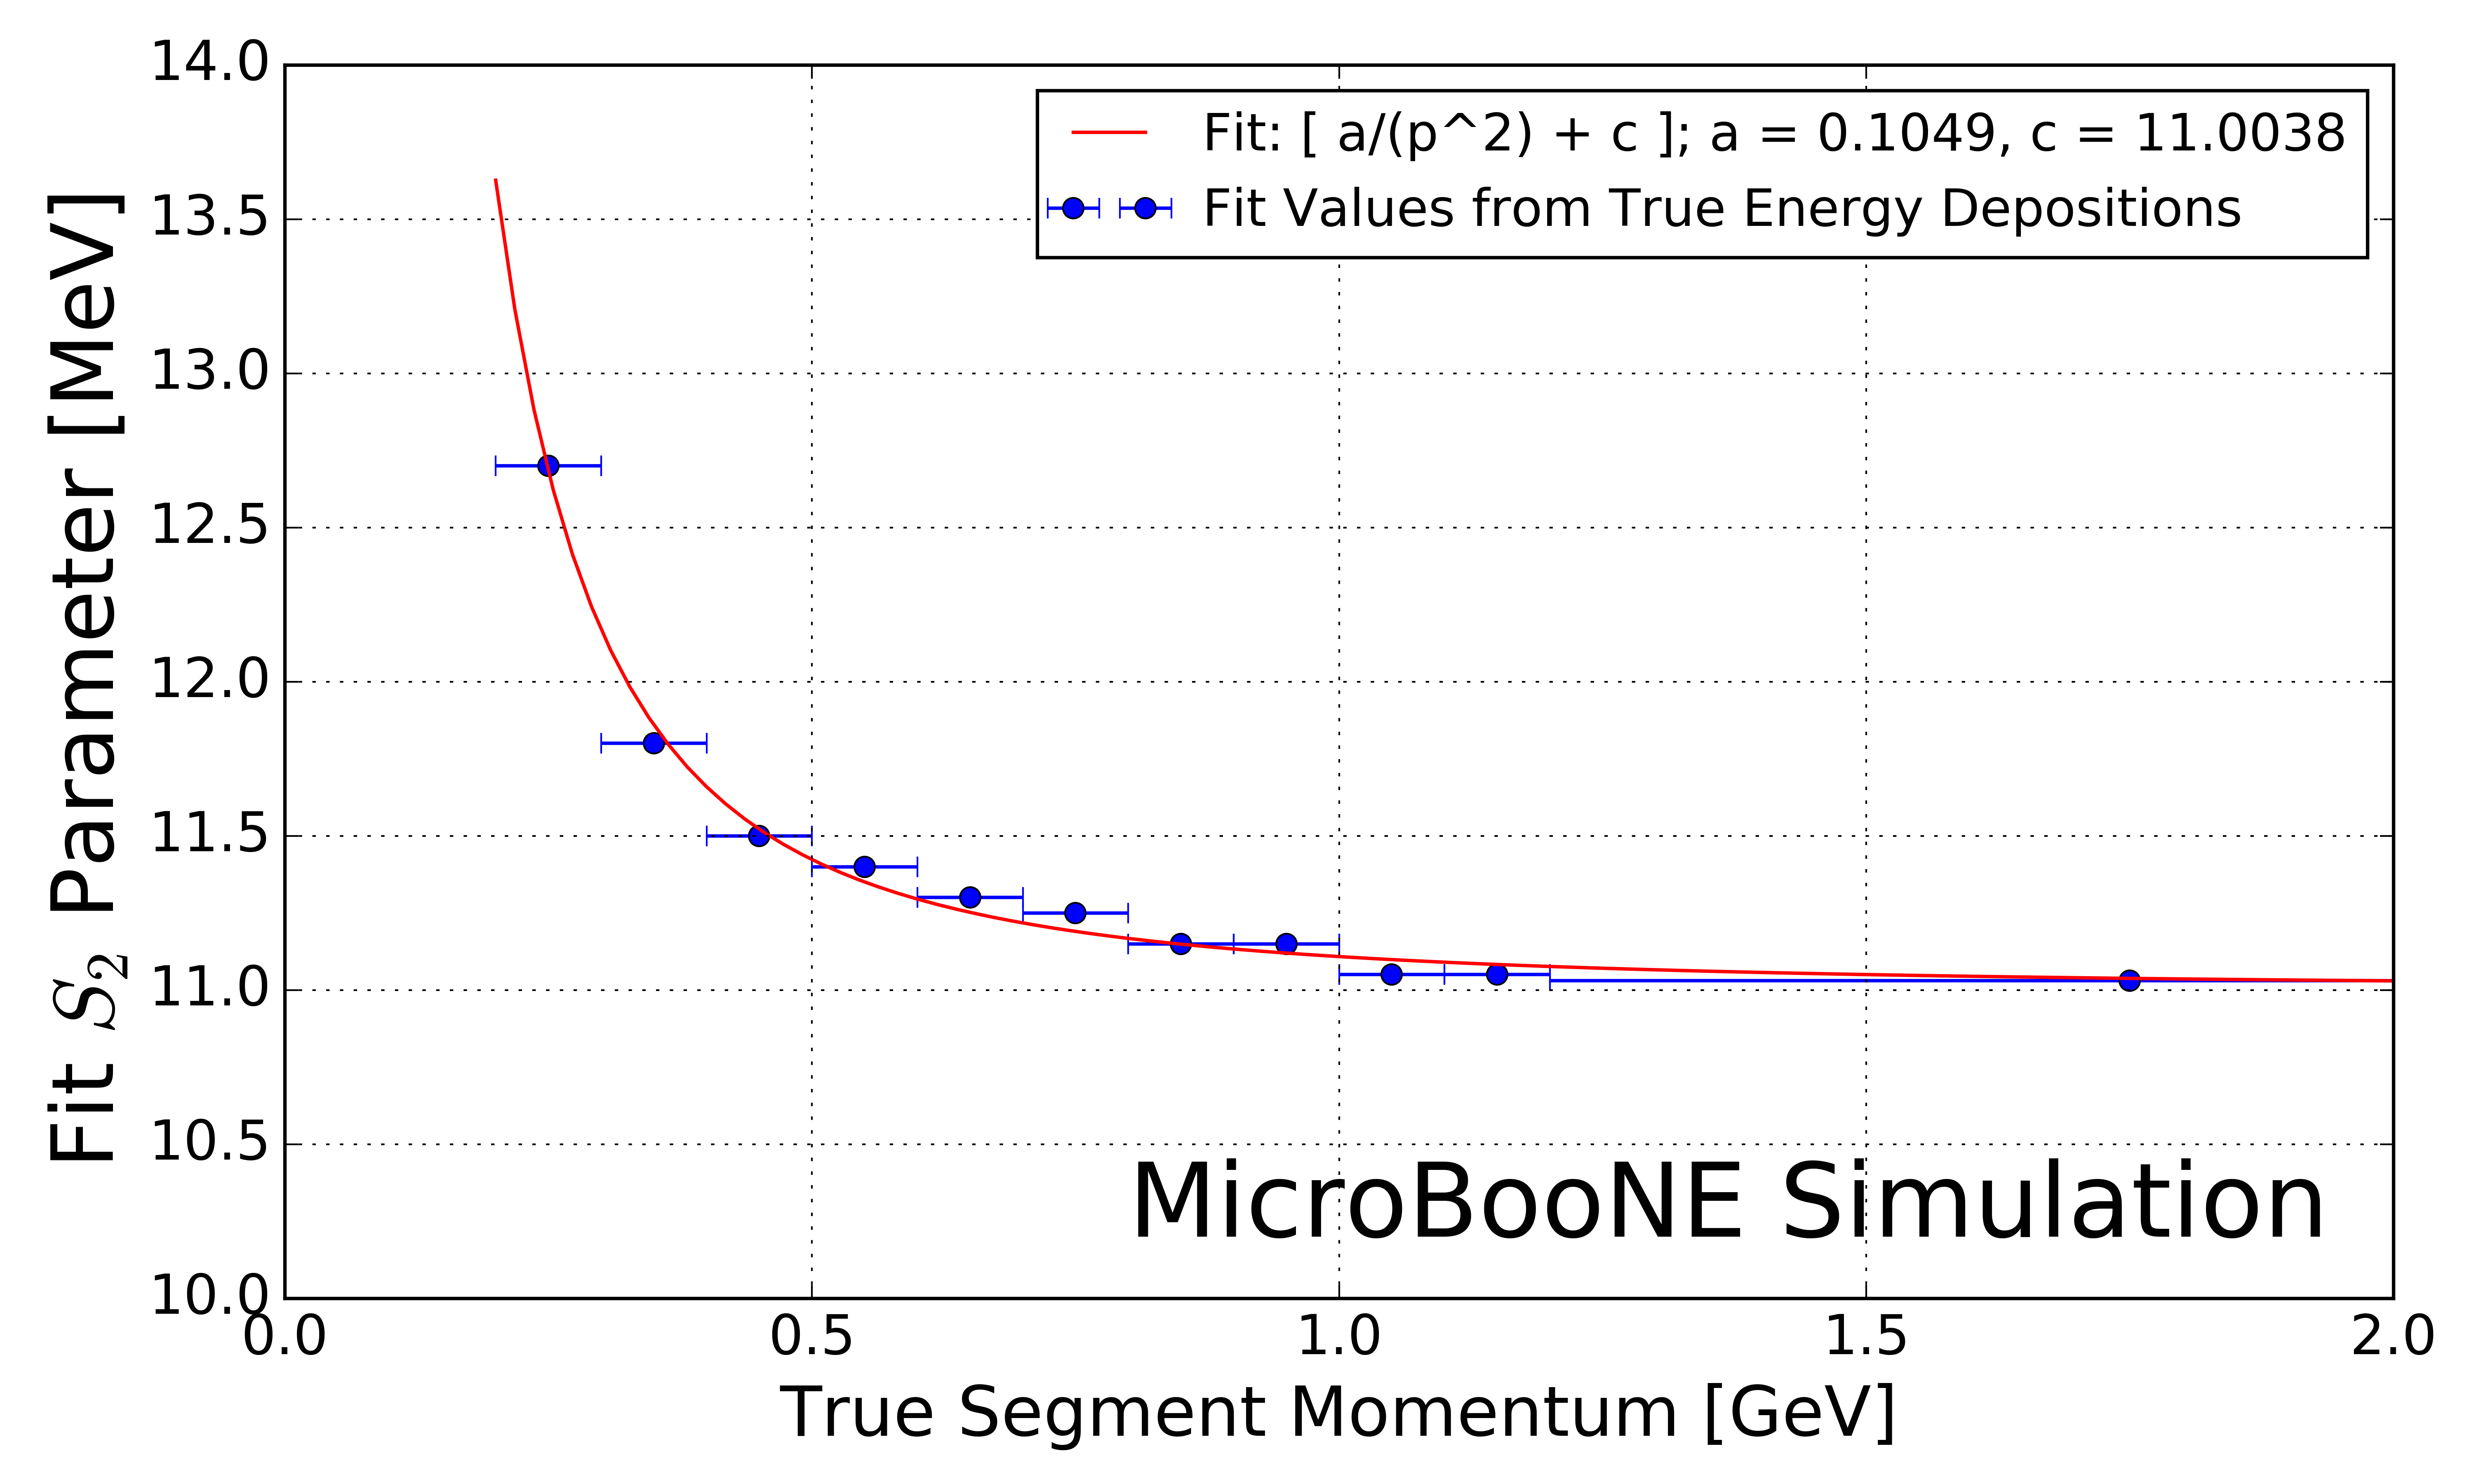
\includegraphics[width=0.9\textwidth]{Figures/highland_constant_optimization_momentumdependent.png}
\end{center}
\caption{Fitted Highland parameter $S_2$ as a function of true segment momentum for ${\ell} = X_0$ simulated muons in the MicroBooNE LArTPC. Blue x- error bars indicate the true momentum bin width with data points drawn at the center of each bin. Shown in red is a fit to these data points with functional form $a\times p^{-2} + c$, with best fit values for parameters $a$ and $c$ shown in the legend.}
\label{retune_highland_fig1}
\end{figure}

The fitted value of $S_2$ is always less than the nominal $13.6\text{ MeV}$ for momentum greater than $0.25\text{ GeV/c}$ and asymptotically approaches a constant at higher momentum (where $\beta = 1$) of about $11.0\text{ MeV}$. The value increases in the momentum region where $\beta < 1$. Shown in red is a fit to these data points with functional form $a\times p^{-2} + c$, with best fit values for floating parameters $a$ and $c$ being $0.105~\text{MeV}^3c^{-2}$ and $11.004\text{ MeV}$ respectively. This functional form is chosen because it fits the data well, and asymptotically approaches a constant value when $\beta$ approaches 1. This function, used as a replacement for the $S_2$ parameter in the Highland formula, will henceforth be referred to as $\kappa(p)$:
\begin{equation}\label{kappa_equation}
\kappa(p) = \frac{0.105}{p^2}\text{ MeV}^3c^{-2} + 11.004\text{ MeV}.
\end{equation}

To visualize the Highland formula for ${\ell} = X_0$ both before and after the $\kappa(p)$ replacement, see figure \ref{retune_highland_fig2}. It is recommended that future LArTPC experiments use this parameterization of the Highland formula, or at the very least conduct their own studies to tune the Highland formula for scattering in argon. This formulation can also be checked in LAr-based test-beam experiments like LArIAT \cite{LARIAT_citation}.\\

\begin{figure}[ht!]
\begin{center}
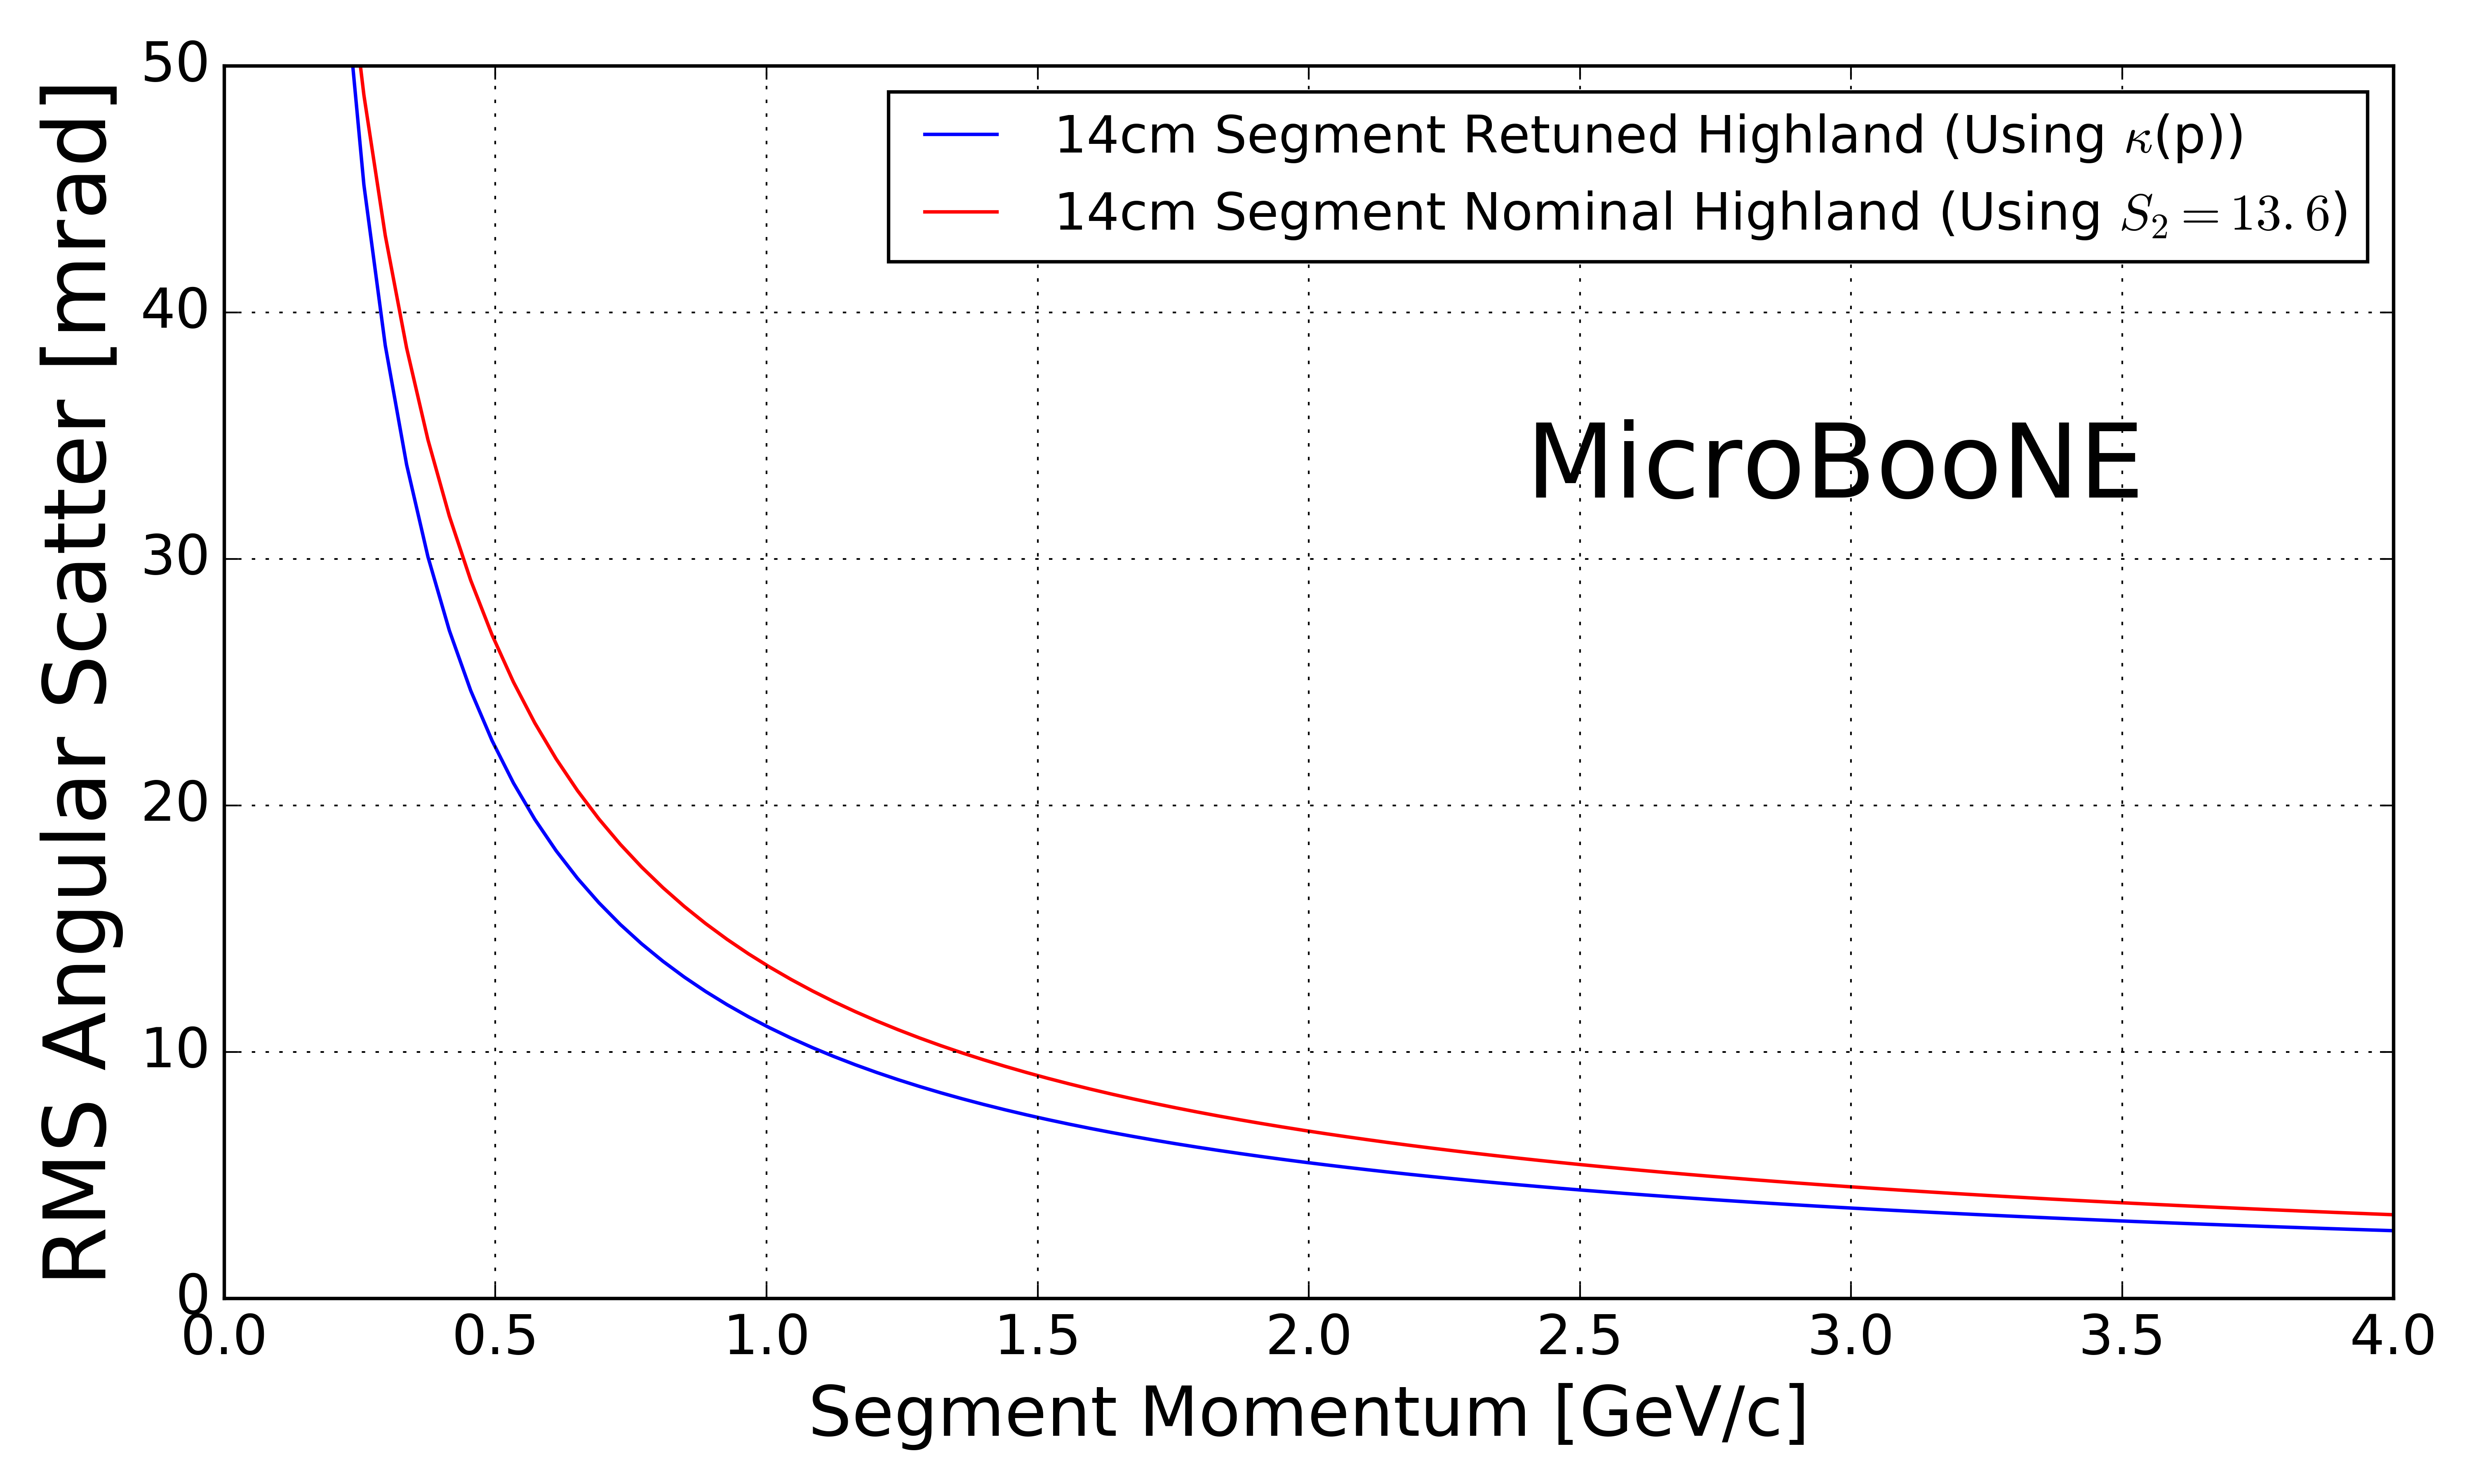
\includegraphics[width=0.9\textwidth]{Figures/highland_formula_visualized_twoforms.png}
\end{center}
\caption{The Highland scattering RMS $\sigma_o^{\text{HL}}$ for 14 cm segment lengths and 0 detector-inherent angular resolution as a function of true momentum before and after tuning. In red is shown equation \ref{highland_simplified} (the nominal Highland formula using $S_2 = 13.6~\text{MeV}$) and in blue is the retuned Highland formula (replacing $S_2$ with $\kappa(p)$).}
\label{retune_highland_fig2}
\end{figure}

With ${\ell} = X_0$, the form of the Highland equation used in this analysis is therefore
\begin{equation}\label{modified_highland_eqtn_kappa}
\sigma_{o}^{\text{RMS}} = \sqrt{ (\sigma_o)^2 + (\sigma_o^{\text{res}})^2} = \sqrt{ \left(\frac{\kappa(p)}{p\beta c}\right)^2 + (\sigma_o^{\text{res}})^2 }.
\end{equation}












\section{MCS implementation using the maximum likelihood method}\label{MCS_technique_section}

This section explains in detail how the phenomenon of multiple Coulomb scattering is used to determine the momentum of a muon track reconstructed in a LArTPC. In general, the approach is as follows:
\begin{enumerate}
\item The three-dimensional track is divided into segments of configurable length.
\item The scattering angles between consecutive segments are measured.
\item Those angles combined with the modified, tuned Highland formula (equation \ref{modified_highland_eqtn_kappa}) are used to build a likelihood that the particle has a specific momentum, taking into account energy loss in upstream segments of the track.
\item The momentum corresponding to the maximum of the likelihood is chosen to be the MCS-computed momentum.
\end{enumerate}
Each of these steps is discussed in detail in the following subsections.\\

% For this analysis, a minimum start-to-end reconstructed track length of 100 cm was used. A minimum length is required to allow for sufficient scatters to measure the momentum. With 100 cm tracks and 10 cm segments (see section \ref{track_segmentation_section}), twenty scattering measurements will ultimately be used to reconstruct the momentum of the particle (see section \ref{scattering_angle_computation_section}).













\subsection{Track segmentation and scattering angle computation}\label{track_segmentation_and_scattering_angle_computation_section}
% The input to the track segmentation routine is a vector of ordered three-dimensional trajectory points (x,y,z) representing the reconstructed track. The points are ordered along the direction of the track, with the first point representing the start of the track, and the last point representing the end of the track. These trajectory points can be determined in a number of ways by different track reconstruction algorithms. In the case of this analysis, the track reconstruction algorithm is named ``pandoraNuPMA" which constructs these three-dimensional trajectory points by combining two-dimensional hits reconstructed from signals on the different wire planes along with timing information from the photomultiplier tubes to reconstruct the third dimension\cite{Marshall:2015rfa}. Note that the tracking resolution in the y- (vertical) and z- (beam) directions are determined by the wire plane spacings, while the resolution in the x- (drift) direction is determined by optical signal timing and is therefore the x- direction resolution is better than that of the y- and z- directions.\\

% Also input to the track segmentation routine is the desired segment length, which is a tunable parameter. In this note, segment lengths are always taken to be 10 cm (based on the findings of Appendix \ref{SegmentLength_MCBNBRecoTrack_section}) except where otherwise explicitly stated. 
Track segmentation refers to the subdivision of three-dimensional reconstructed trajectory points of a reconstructed track into portions of definite length. In this analysis, the tracks are automatically reconstructed by the ``pandoraNuPMA" projection matching algorithm \cite{Marshall:2015rfa}. The algorithm constructs the three-dimensional trajectory points by combining two-dimensional hits reconstructed from signals on the different wire planes along with timing information from the photomultiplier tubes. The segmentation process begins at the start of the track, and iterates through the trajectory points in order, defining segment start and stop points based on the straight-line distance between them. There is no overlap between segments. Given the subset of the three-dimensional trajectory points that corresponds to one segment of the track, a three-dimensional linear fit is applied to the data points, weighting all trajectory points equally in the fit. In this analysis, a segment length of 14 cm is used, which is a tunable parameter that has been chosen as described in the derivation of $\kappa(p)$ (equation \ref{kappa_equation}).\\

With the segments defined, the scattering angles between the linear fits from adjacent segments are computed. A coordinate transformation is performed such that the $z'$ direction is oriented along the direction of the linear fit to the first of the segment pair. The $x'$ and $y'$ coordinates are chosen such that all of $x'$, $y'$, and $z'$ are mutually orthogonal and right-handed, as shown in figure \ref{mcs_nocap_fig}. The scattering angles with respect to the $x'$ direction and the $y'$ direction are computed as input to the MCS algorithm. Only the scattering angle with respect to the $x'$ direction is drawn in figure \ref{mcs_nocap_fig}.



% This routine within the MCS code takes as input the vector of length $n$ (where $n$ is the number of segments for the track) containing the direction cosines at the start of each segment. In general, the algorithm iterates over consecutive pairs of segments (the segmentation routine is described in section \ref{track_segmentation_section}) and computes angular scatters between each, and stores them for later use by a future subroutine. This code is more complicated than just taking the dot product between consecutive direction cosines to find the total angular scatter between segments because the Highland formula is derived from scattering independently in the two directions orthogonal to the direction of the track. For this reason, this subroutine performs a coordinate transformation for each pair of segments such that the direction of first of the two segments is along the $z'$ direction, as drawn in figure \ref{mcs_nocap_fig}. With the $z'$ direction defined as such, $x'$ and $y'$ directions are chosen such that all of $x'$, $y'$, and $z'$ are mutually orthogonal, again shown in figure \ref{mcs_nocap_fig}\footnote{Note that at this point, all of $x'$, $y'$, and $z'$ are different than the detector coordinates, $x$, $y$, and $z$ which correspond to drift direction, vertical direction, and beam direction respectively.}. The scattering angles both in the $x'$ and $y'$ planes are then computed for each consecutive pairs of segments\footnote{Both of these scattering angles are used downstream in the MCS algorithm, and therefore the choice of $x'$ and $y'$ are not important.}. After this routine, a vector of length $2n$ is stored containing the scattering angles in the $x'$ plane as well as in the $y'$ plane. These scattering angles are what are input into the maximum likelihood routine to determine track momentum.














\subsection{Maximum likelihood theory}\label{likelihood_theory_section}

The normal probability distribution for a scattering angle in either the $x'$ or $y'$ direction, $\Delta\theta$, with an expected Gaussian uncertainty $\sigma_o$ and mean of zero is given by
\begin{equation}
f_X(\Delta\theta) = (2\pi\sigma_o^2)^{-\frac{1}{2}}\exp\left[-\frac{1}{2}\left(\frac{\Delta\theta}{\sigma_o}\right)^2\right].
\end{equation}

Here, $\sigma_o$ is the RMS angular deflection computed by the modified, tuned Highland formula (equation \ref{modified_highland_eqtn_kappa}), which is a function of the momentum and the length of that segment. Since energy is lost between segments along the track, $\sigma_o$ increases for each angular measurement along the track. We therefore replace $\sigma_o$ with $\sigma_{o,j}$, where $j$ is an index representative of the segment. \newline

To obtain the likelihood, we take the product of $f_X(\Delta\theta_j)$ over all $n$ of the $\Delta\theta_j$ segment-to-segment scatters along the track. This product can be written as
\begin{equation}
L(\sigma_{o,1},...,\sigma_{o,n};\Delta\theta_1,...,\Delta\theta_n) = (2\pi)^{-\frac{n}{2}}\times\prod_{j=1}^{n}(\sigma_{o,j})^{-1} \times \exp\left[-\frac{1}{2}\sum_{j=1}^{n}\left(\frac{\Delta\theta_j}{\sigma_{o,j}}\right)^2\right].
\end{equation}

Rather than maximizing the likelihood it is more computationally convenient to instead minimize the negative log likelihood. Inverting the sign and taking $\ln(L)$ gives an expression that is related to a $\chi^2$ variable:
\begin{equation}\label{leo_llhd_eqtn}
-l(\mu_o;\sigma_{o,1},...,\sigma_{o,n};\Delta\theta_1,...,\Delta\theta_n) = -\ln(L) = \frac{n}{2}\ln(2\pi) + \sum_{j=1}^{n}\ln(\sigma_{o,j}) + \frac{1}{2}\sum_{j=1}^{n}\left(\frac{\Delta\theta_j}{\sigma_{o,j}}\right)^2
\end{equation}

% The negative log likelihood for one specific segment's angular scatter $\Delta\theta_j$ given an expected scattering RMS $\sigma_{o,j}$ is given by the following equation
% \begin{equation}\label{negative_llh_eqtn}
% -l(\mu_o, \sigma_{o,j}, \Delta\theta_j) = \frac{1}{2}ln(2\pi) + ln(\sigma_{o,j}) + \frac{1}{2}\frac{(\Delta\theta_j-\mu_o)^2}{(\sigma_{o,j})^2}
% \end{equation}

% In general, Equation \ref{negative_llh_eqtn} is evaluated for each segment in a track given a postulated full track momentum, and the sum of these terms is used to determine the likelihood that the postulated track momentum is correct for that track.











\subsection{Maximum likelihood implementation}\label{maximum_likelihood_section}

Given a set of angular deflections in the $x'$ and $y'$ directions for each segment as described in section \ref{track_segmentation_and_scattering_angle_computation_section} a scan is done over the postulated initial energy, $E_t$, in steps of 1 MeV up to 7.5 GeV. The step with the smallest negative log likelihood (equation \ref{leo_llhd_eqtn}) is chosen as the MCS energy. Equation \ref{leo_llhd_eqtn} includes a $\sigma_{o,j}$ term that changes for consecutive segments because their associated energy is decreasing. The energy of the $j$th segment is related to $E_t$ by

\begin{equation}\label{segment_E_equation}
E_{j} = E_t - \Delta E_{j},
\end{equation}

\noindent where $\Delta E_{j}$ is the energy loss upstream of this segment, computed by integrating the muon stopping power curve given by the Bethe-Bloch equation described by the Particle Data Group (PDG) \cite{stoppingpowersource} along the length of track upstream of this segment. Equation \ref{segment_E_equation} introduces a minimum allowable track energy determined by the range of the track, as $E_{j}$ must remain positive. The use of the Bethe-Bloch equation to determine $\Delta E_{j}$ impacts the MCS algorithm resolution for fully contained tracks, but does not for exiting tracks where much of the ionization energy loss is not visible. This value of segment energy, $E_{j}$, is converted to a momentum $p$ with the relativistic energy-momentum relation assuming the muon mass, and is then used to predict the RMS angular scatter for that segment ($\sigma_o$) by way of equation \ref{modified_highland_eqtn_kappa}. 

\section{Range-based energy validation from simulation}\label{Range_Energy_Validation_section}
In order to quantify the performance of the MCS energy estimation method on fully contained muons in data, an independent determination of energy is needed. Range-based energy, $E_{\text{range}}$ is used here because the true energy $E_{\text{true}}$ will not be known in analyzing detector data. The stopping power of muons in liquid argon is well described by the continuous slowing-down approximation (CSDA) by the particle data group, and agrees with data at the sub-percent level \cite{MIPenergysource} \cite{PDG_spline_table} \cite{NISTdata}. By using a linear interpolation between points in the stopping power table of ref. \cite{PDG_spline_table}, the length of a track can be used to reconstruct the muon's total energy with good accuracy. A simulated sample of fully contained BNB neutrino-induced muons longer than one meter is used to quantify the bias and resolution for the range-based energy estimation technique. The range is defined as the straight-line distance between the true starting point and true stopping point of a muon, even though the trajectories are not perfectly straight lines. The bias and resolution are computed in bins of true total energy of the muons by fitting a Gaussian function to a distribution of the fractional energy difference $(E_{\text{Range}}-E_{\text{True}})/(E_{\text{True}})$ in each bin. The mean of each Gaussian yields the bias for that true energy bin, and the width indicates the resolution. Figure \ref{true_range_bias_resolution_MCTrack_fig} shows the bias and resolution for the range-based energy reconstruction method. The bias is negligible and the resolution for this method of energy reconstruction increases slightly with true muon energy but remains on the order of (2-4)\%. This result demonstrates that range-based energy (and therefore range-based momentum) is a good estimator of the true energy (momentum) of a reconstructed contained muon track in data, assuming that the track is well reconstructed in terms of length.

\begin{figure}
\centering
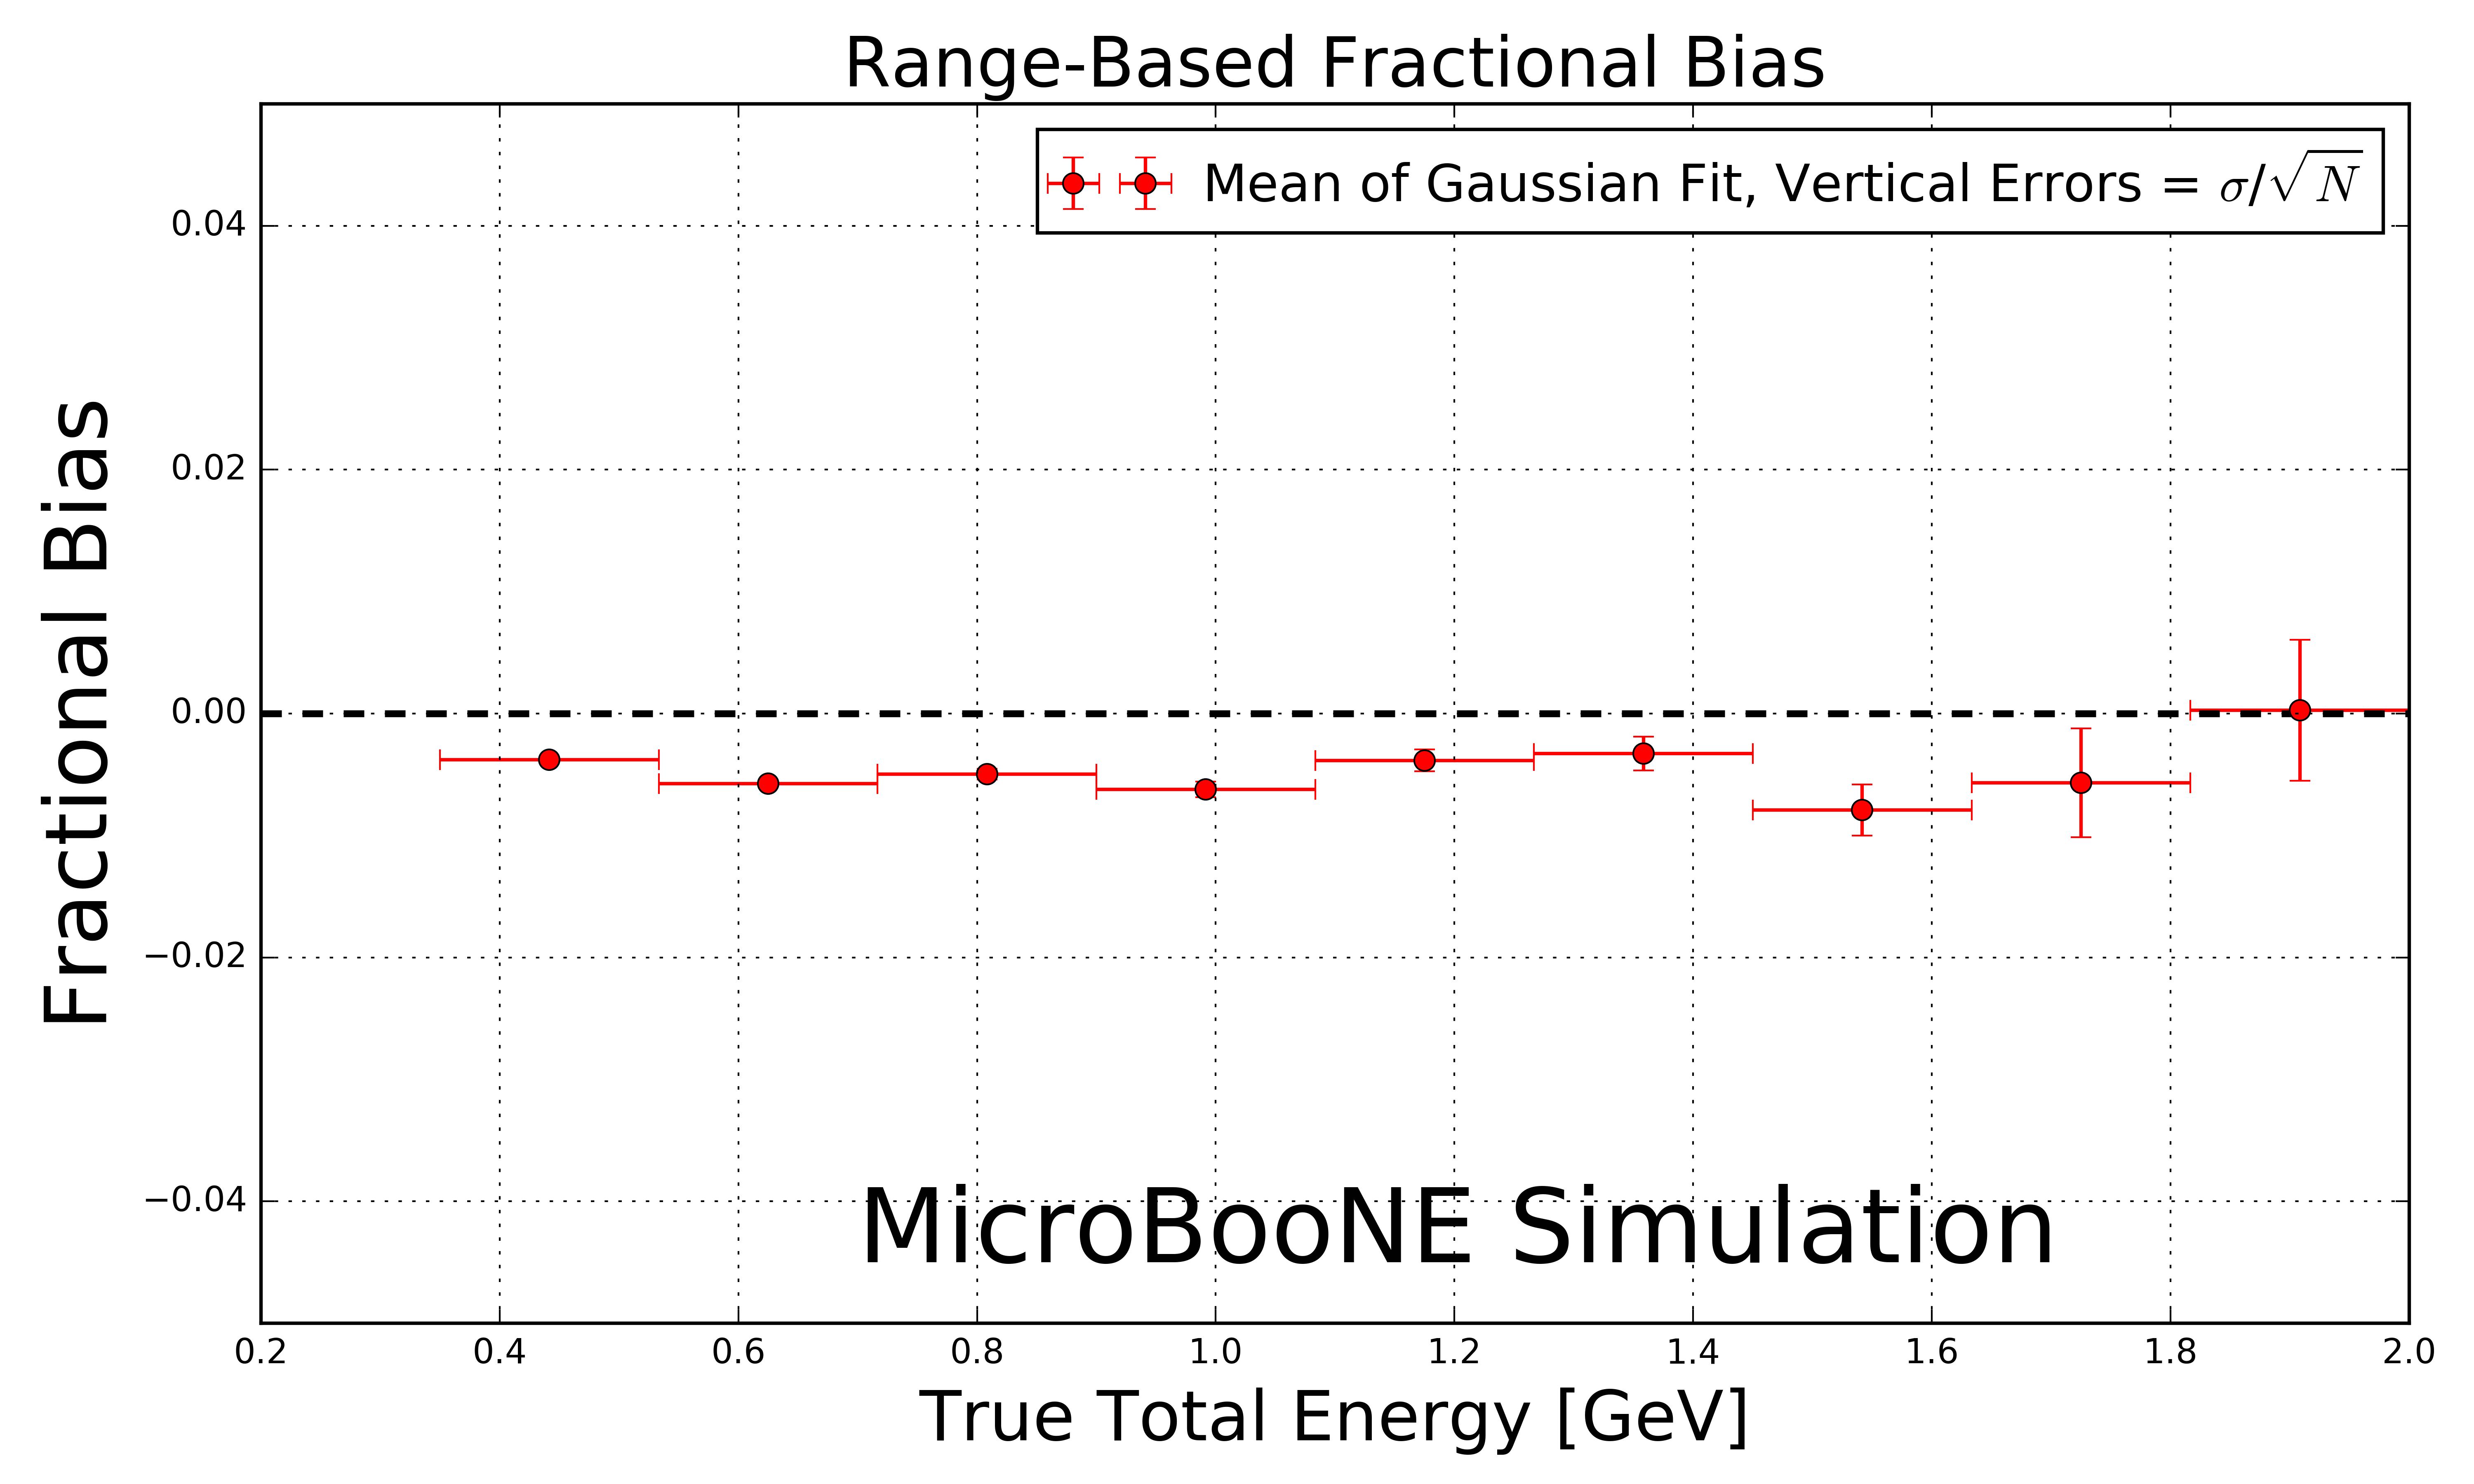
\includegraphics[width=0.9\textwidth]
	{Figures/true_range_bias_MCBNBMCTrack.png}
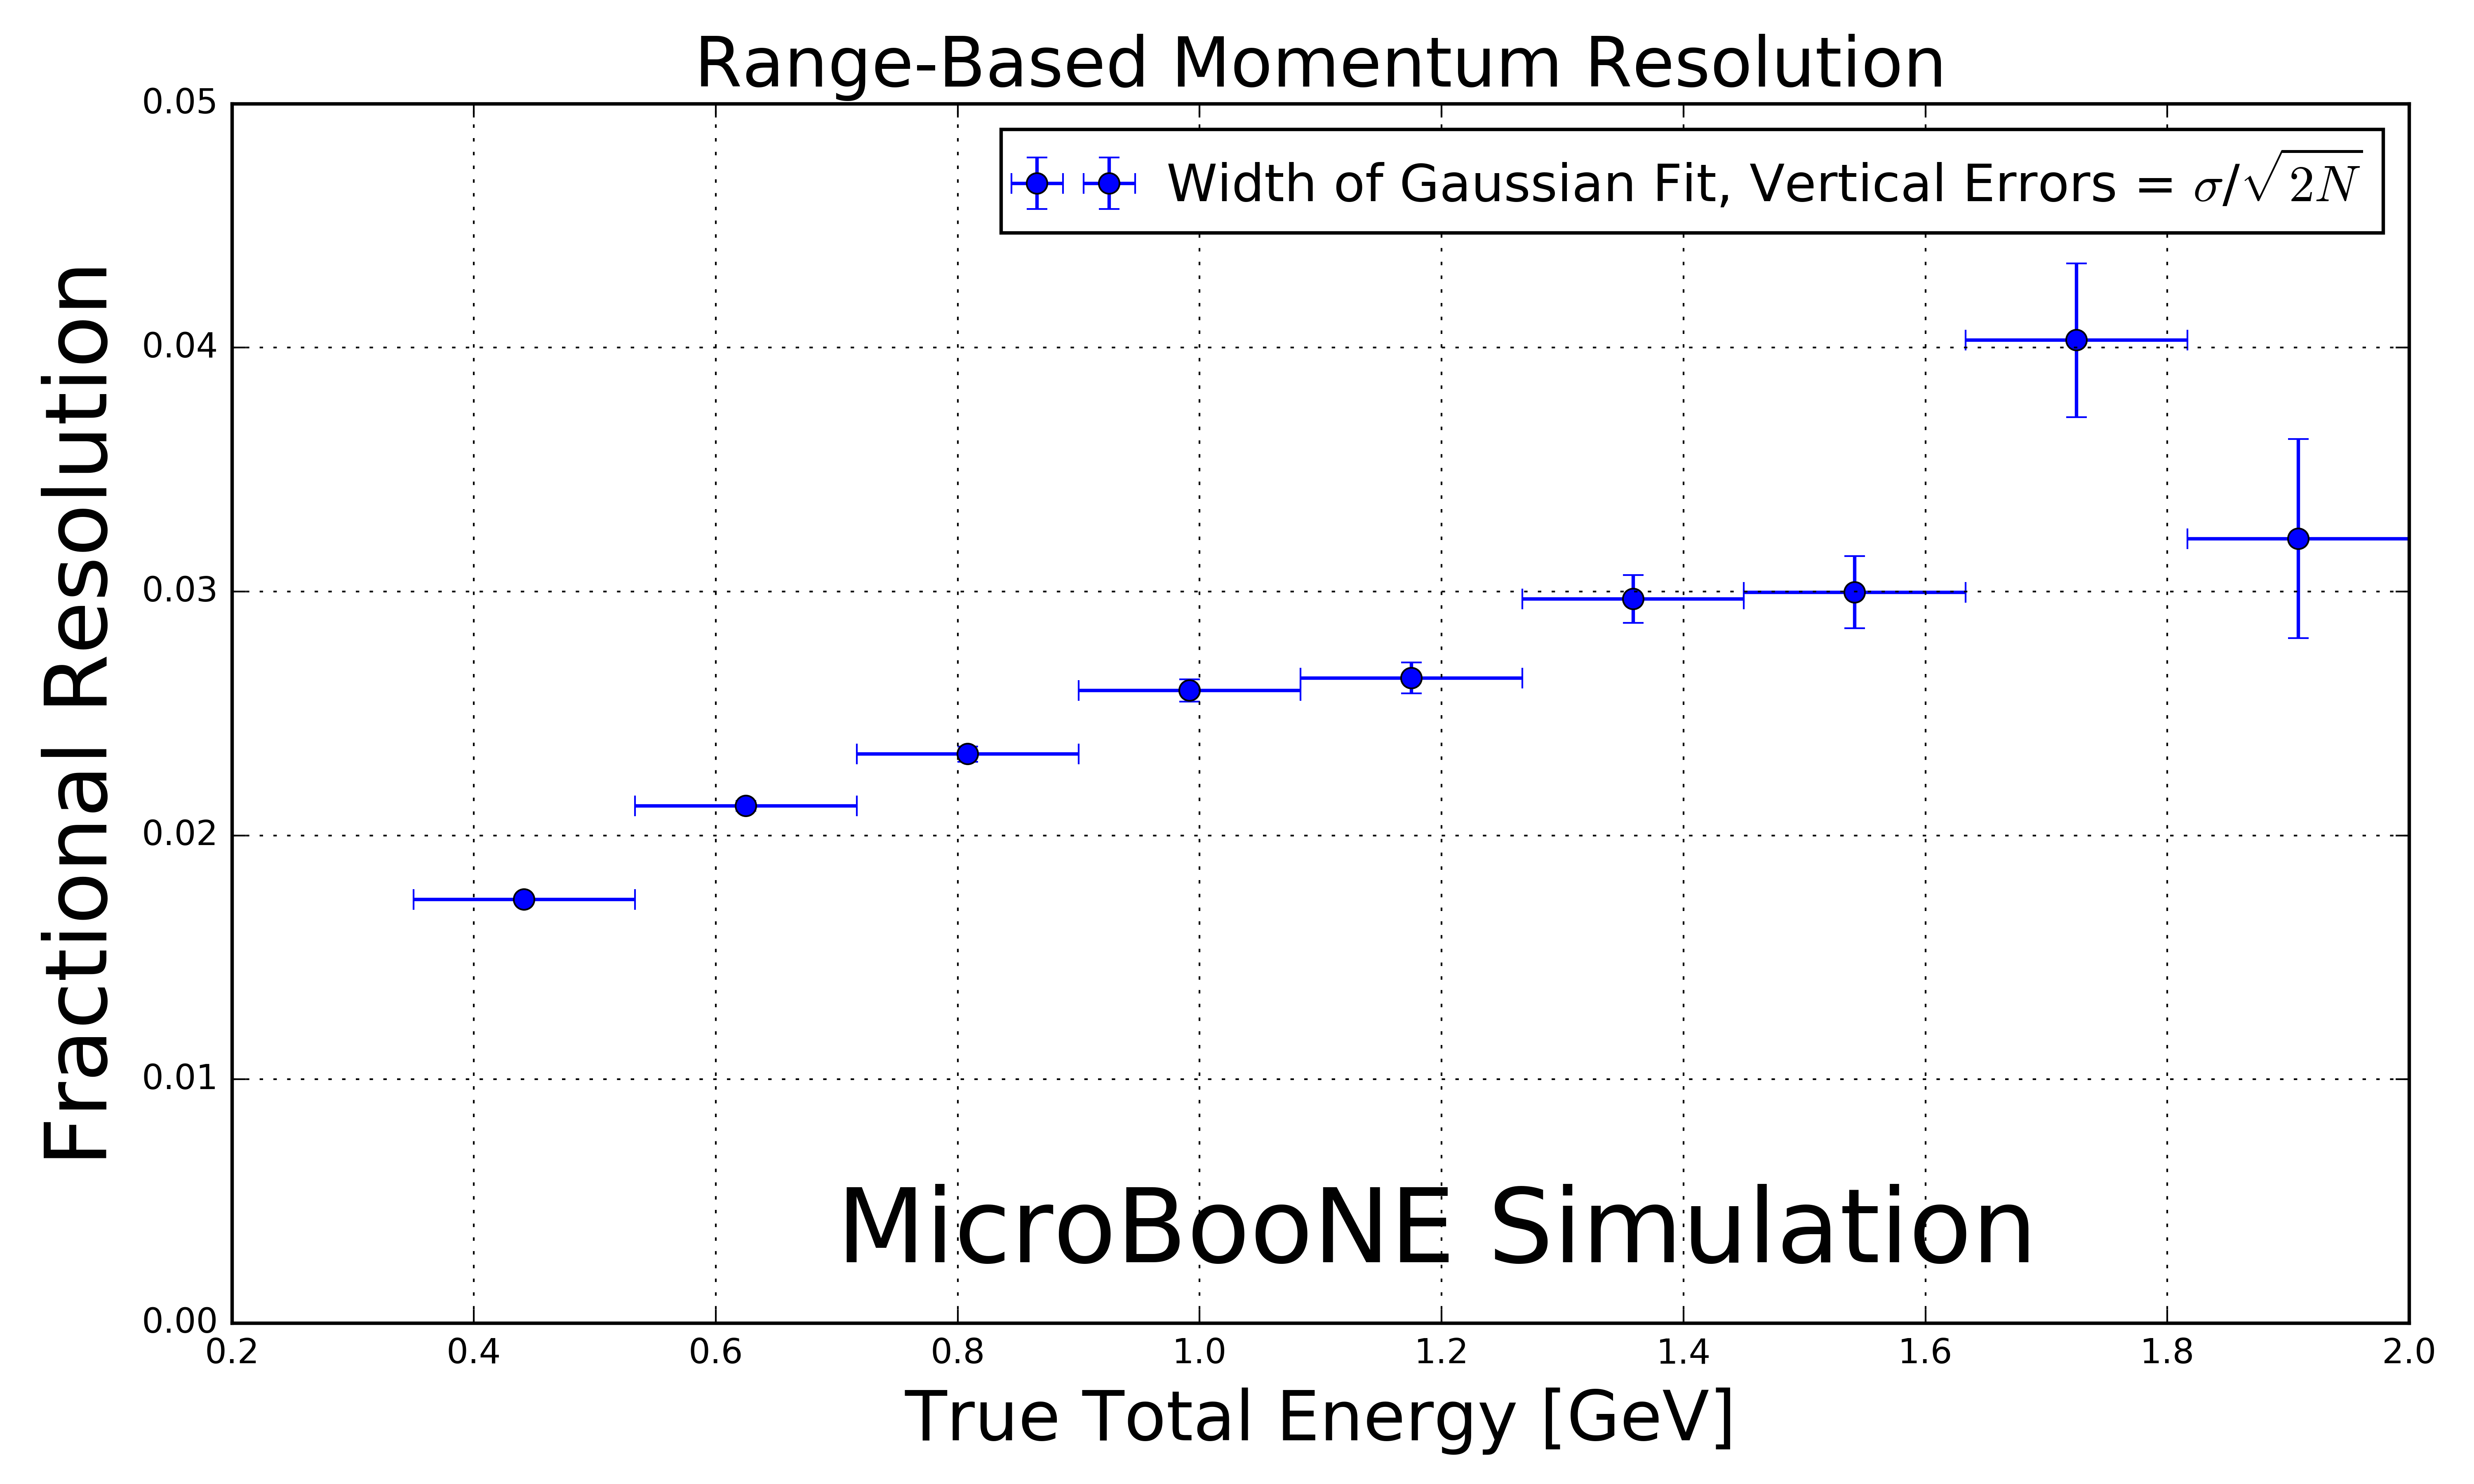
\includegraphics[width=0.9\textwidth]
	{Figures/true_range_resolution_MCBNBMCTrack.png}
\caption{Range-based energy fractional bias (a) and resolution (b) from a sample of simulated fully contained BNB neutrino-induced muons using true starting and stopping positions of the track. The bias is less than 1\% and the resolution is below $\approx$4\%.}
\label{true_range_bias_resolution_MCTrack_fig}
\end{figure}






\section{MCS performance on beam neutrino-induced muons in MicroBooNE data}\label{data_performance_section}

\subsection{Input sample}\label{input_sample_section}
This part of the analysis is based on triggered neutrino interaction events in MicroBooNE corresponding to $\approx 5 \times 10^{19}$ protons on target, which is a small subset ($<$10\%) of the nominal protons on target scheduled to be delivered to the detector. These events are run through a fully automated reconstruction chain that produces reconstructed objects including three-dimensional neutrino interaction points (vertices), three-dimensional tracks (as described in section \ref{track_segmentation_and_scattering_angle_computation_section}) for each outgoing secondary particle from the interaction, and PMT-reconstructed optical flashes from the interaction scintillation light. The fiducial volume used in this analysis is defined in section \ref{sec:intro}.

\subsection{Event selection}
The following selection criteria are placed on the reconstructed objects to select $\nu_\mu$ charged-current interactions in which a candidate muon track exiting the interaction vertex is fully contained within the fiducial volume:
\begin{enumerate}
\item The event must have at least one bright optical flash, reconstructed from PMT timing signals, in coincidence with the expected BNB-neutrino arrival time.
\item Two or more reconstructed tracks must originate from the same reconstructed vertex within the fiducial volume.
\item The $z$ coordinate of the optical flash, as determined by the pulse height and timing of signals in the 32 PMTs, must be within 70 cm of any point on the $z$ projection of the candidate muon track.
\item For events with exactly two tracks originating from the vertex, additional calorimetric criteria are applied to mitigate backgrounds from cosmic muons that arrive in time with the passage of the beam, then stop and decay to an electron that is reconstructed as a track.
\item The longest track originating from the vertex is assumed to be a muon, and it must be fully contained within the fiducial volume.
\item The length of the longest track must be $>$1~m in order to have sufficient sampling points in the MCS likelihood to obtain a reasonable estimate of momentum.
\end{enumerate}

These selection criteria are chosen to select a sample of tracks with high purity. In this sample of MicroBooNE data, 598 events (tracks) remain after all selections. The low statistics in this sample is due to the size of the input sample and the low efficiency associated with the applied high-purity selection, described in section \ref{input_sample_section}. Each of these events (tracks) was scanned by hand with a 2D interactive event display showing the raw wire signals of the interaction from each wire plane, with the 2D projection of the reconstructed muon track and vertex overlaid. The scanning was done to ensure the track is well reconstructed with start point close to the reconstructed vertex and end point close to the end of the visible wire-signal track in all three planes. During the scanning, obvious mis-identification topologies were removed. An example of such a topology is a stopping cosmic-ray muon decaying into an electron. After rejecting events (tracks) based on hand scanning, 396 tracks remain for analysis.


\subsection{Validation of the Highland formula}\label{highland_validation_section}
The Highland formula indicates that distributions of angular deviations of the track, segment by segment, in both the $x'$ and $y'$ directions divided by the width predicted from the Highland equation $\sigma_o^{\text{RMS}}$ (equation \ref{modified_highland_eqtn_kappa}) should be Gaussian with a width of unity. In order to calculate the momentum $p$ in the Highland equation, $p$ for each segment is computed with equation \ref{segment_E_equation}, where $E_t$ comes from the converged MCS-computed momentum of the track. For each consecutive pair of segments in this sample of 396 tracks, the angular scatter divided by the Highland expected RMS (including detector resolution term, $\sigma_o^{\text{res}}$) is an entry in the area-normalized distribution shown in figure \ref{Highland_validation_fig}. These 396 tracks have on average 12 segments each, therefore this histogram has approximately $396\times12\times2=9504$ entries. The additional factor of 2 comes from angular scatters both in the $x'$ and $y'$ directions. The distribution has an RMS of unity, thus validating the MCS technique used in this analysis.

\begin{figure}[ht!]
\centering
	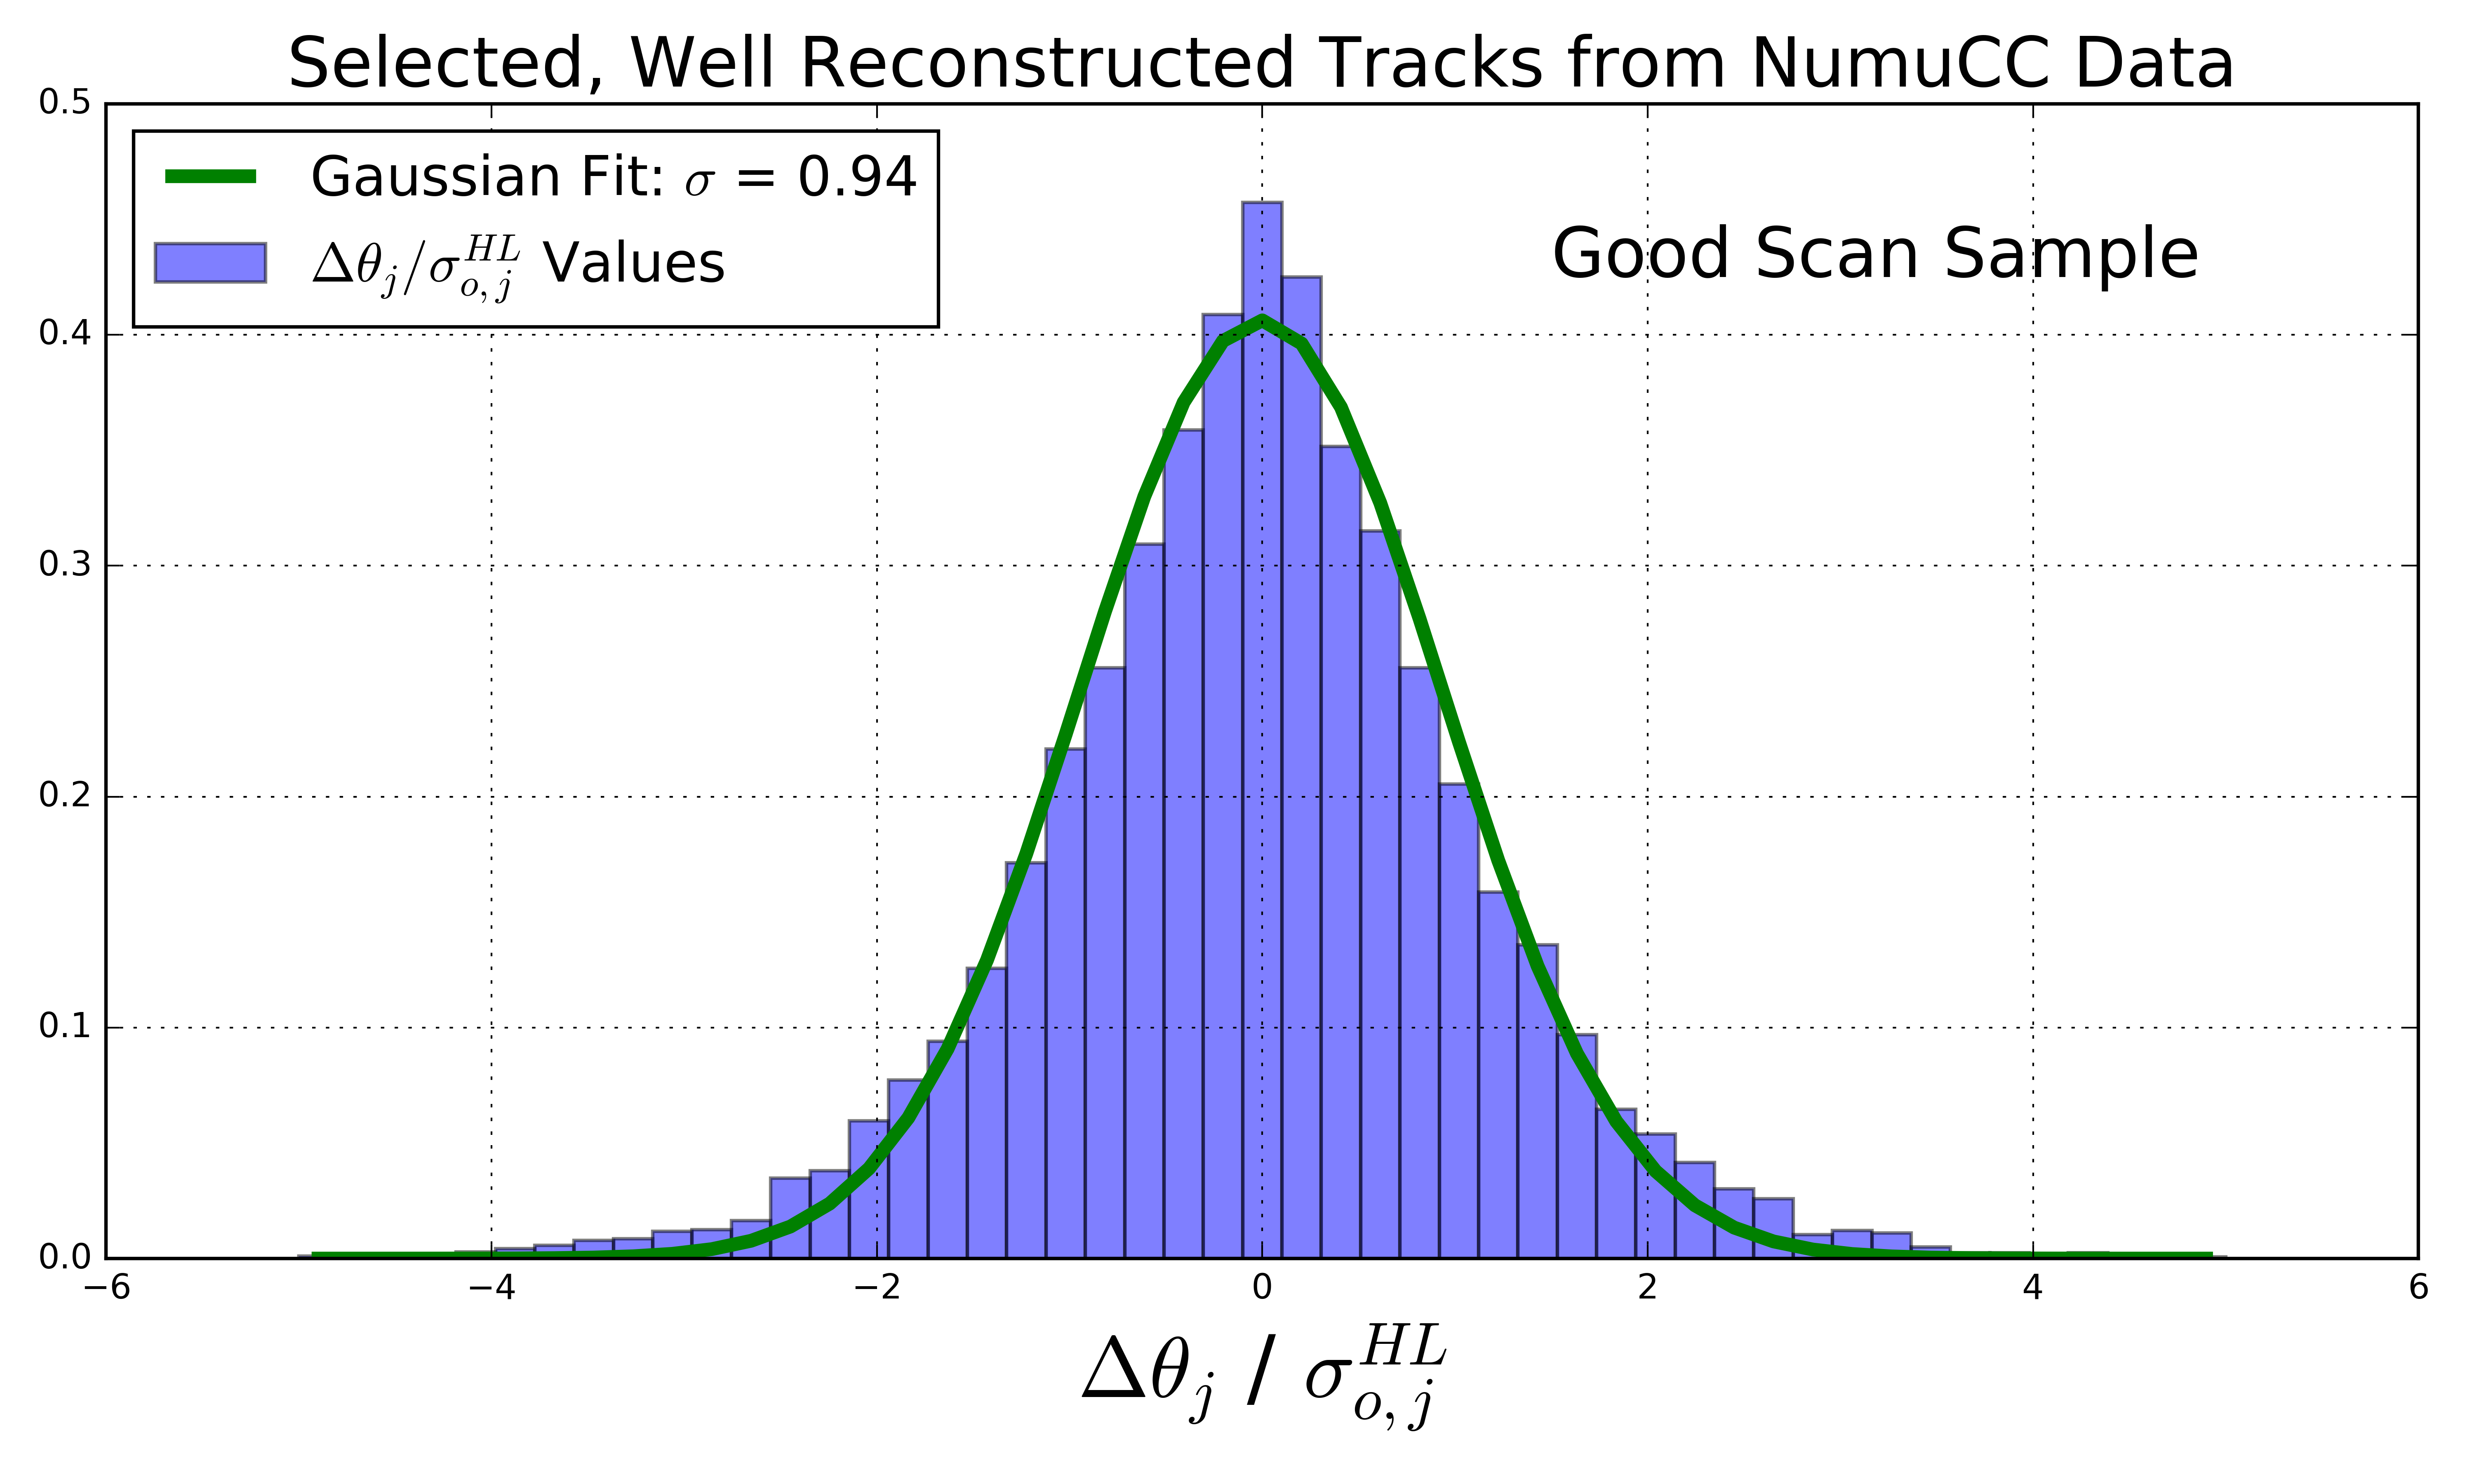
\includegraphics[width=0.9\textwidth]{Figures/Highland_validation_DataBNBSelectedRecoTrack_goodscan.png} \\
\caption{Segment-to-segment measured angular scatters in both the $x'$ and $y'$ directions divided by the width $\sigma_o^{\text{RMS}}$ predicted by the Highland formula (equation \ref{highland_eqtn}) for the automatically selected beam neutrino-induced fully contained muon sample in MicroBooNE data after hand scanning to remove poorly reconstructed tracks and obvious mis-identification topologies.}\label{Highland_validation_fig}
\end{figure}


\subsection{MCS momentum validation}\label{MCS_Momentum_Validation_DataRecoTrack_section}

MCS momentum versus range-based momentum for this sample of 396 tracks is shown in figure \ref{realdata_goodhandscan_fig}. The fractional bias and resolution as a function of range-based momentum for this sample is shown in figure \ref{MCS_range_bias_resolution_DataRecoTrack_fig}. In order to compute this bias and resolution, distributions of fractional inverse momentum difference $(p_{\text{MCS}}^{-1} - p_{\text{Range}}^{-1})/(p_{\text{Range}}^{-1})$ in bins of range-based momentum $p_{\text{Range}}$ are fit to Gaussian functions, where the mean of the fit determines the bias while the width of the fit determines the resolution for that bin. Inverse momentum is used here because the binned distributions are more Gaussian since the Highland formula measures inverse momentum in terms of track angles that have reasonably Gaussian errors. Simply using the mean and RMS of the binned distributions yields similar results. Also shown in this figure are the bias and resolutions for a simulated sample consisting of a full BNB simulation with CORSIKA-generated \cite{corsika_ref} cosmic overlays passed through an identical reconstruction and event selection chain. Rather than hand scanning this sample, true simulation information is used by requiring the longest reconstructed track to be matched well to the true starting and stopping point of the $\nu_\mu$CC muon. This removes any mis-identifications or interference from the simulated cosmics. 
%These resolutions on the order of 10\% are consistent with the Mote Carlo Kalman filter results presented by the ICARUS collaboration in this momentum range \cite{icarus_mcs_paper} as summarized in Table \ref{icarus_comparison_table}.\\

\begin{figure}[ht!]
\centering
	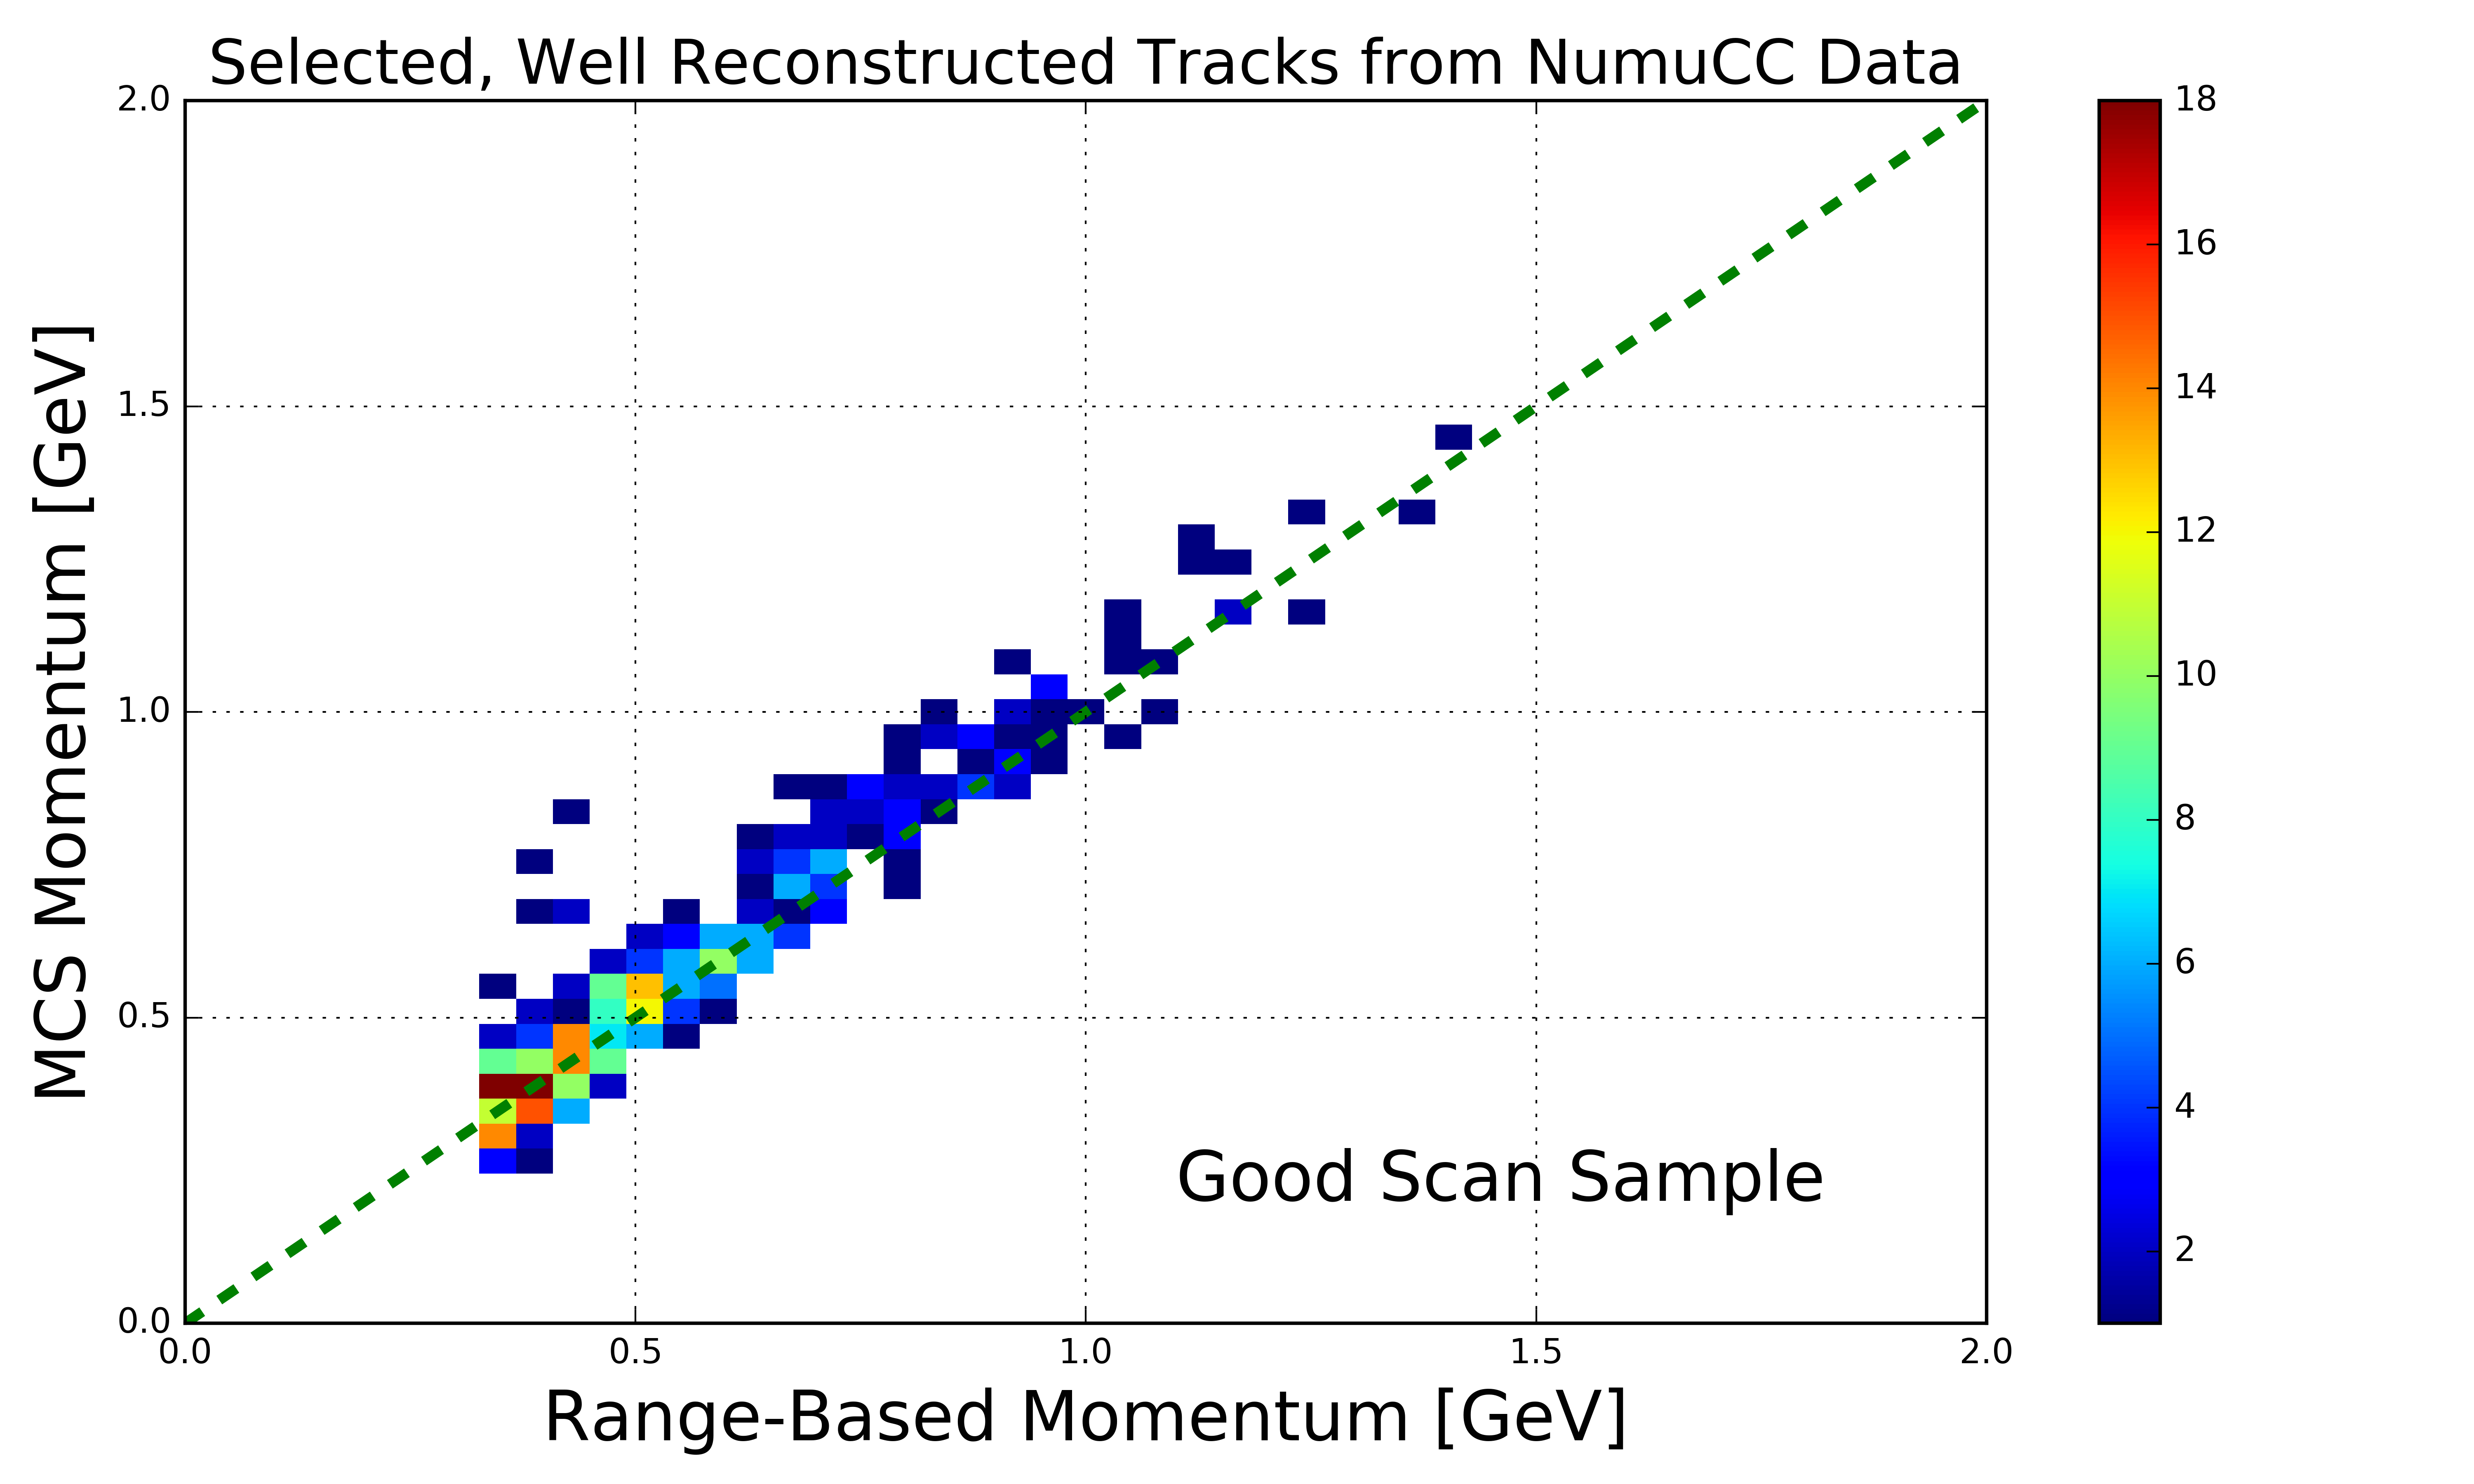
\includegraphics[width=0.9\textwidth]{Figures/MCS_range_momentum_DataRecoTracks_goodhandscan.png} \\
\caption{MCS-computed momentum versus range momentum for the automatically selected beam neutrino-induced fully contained muon sample in MicroBooNE data after hand scanning to remove poorly reconstructed tracks and obvious mis-identification topologies. The color (z) scale indicates number of tracks.}\label{realdata_goodhandscan_fig}
\end{figure}

% \begin{table}[htbp]
% \centering
% \caption{\label{icarus_comparison_table} MicroBooNE maximum-likelihood based MCS fractional resolution on simulation as compared to published ICARUS Kalman Filter based MCS fractional resolution on simulation \cite{icarus_mcs_paper} as manually extrapolated from Figure 7 in the cited publication.}
% \smallskip
% \begin{tabular}{|c|c|c|}
% \hline
%  & $p_{true}$ = 0.5 GeV& $p_{true}$ = 1.0 GeV\\
% \hline
% ICARUS & 12\% & 10\%\\
% MicroBooNE & 9\% & 6\%\\
% \hline
% \end{tabular}
% \end{table}



\begin{figure}
\centering
	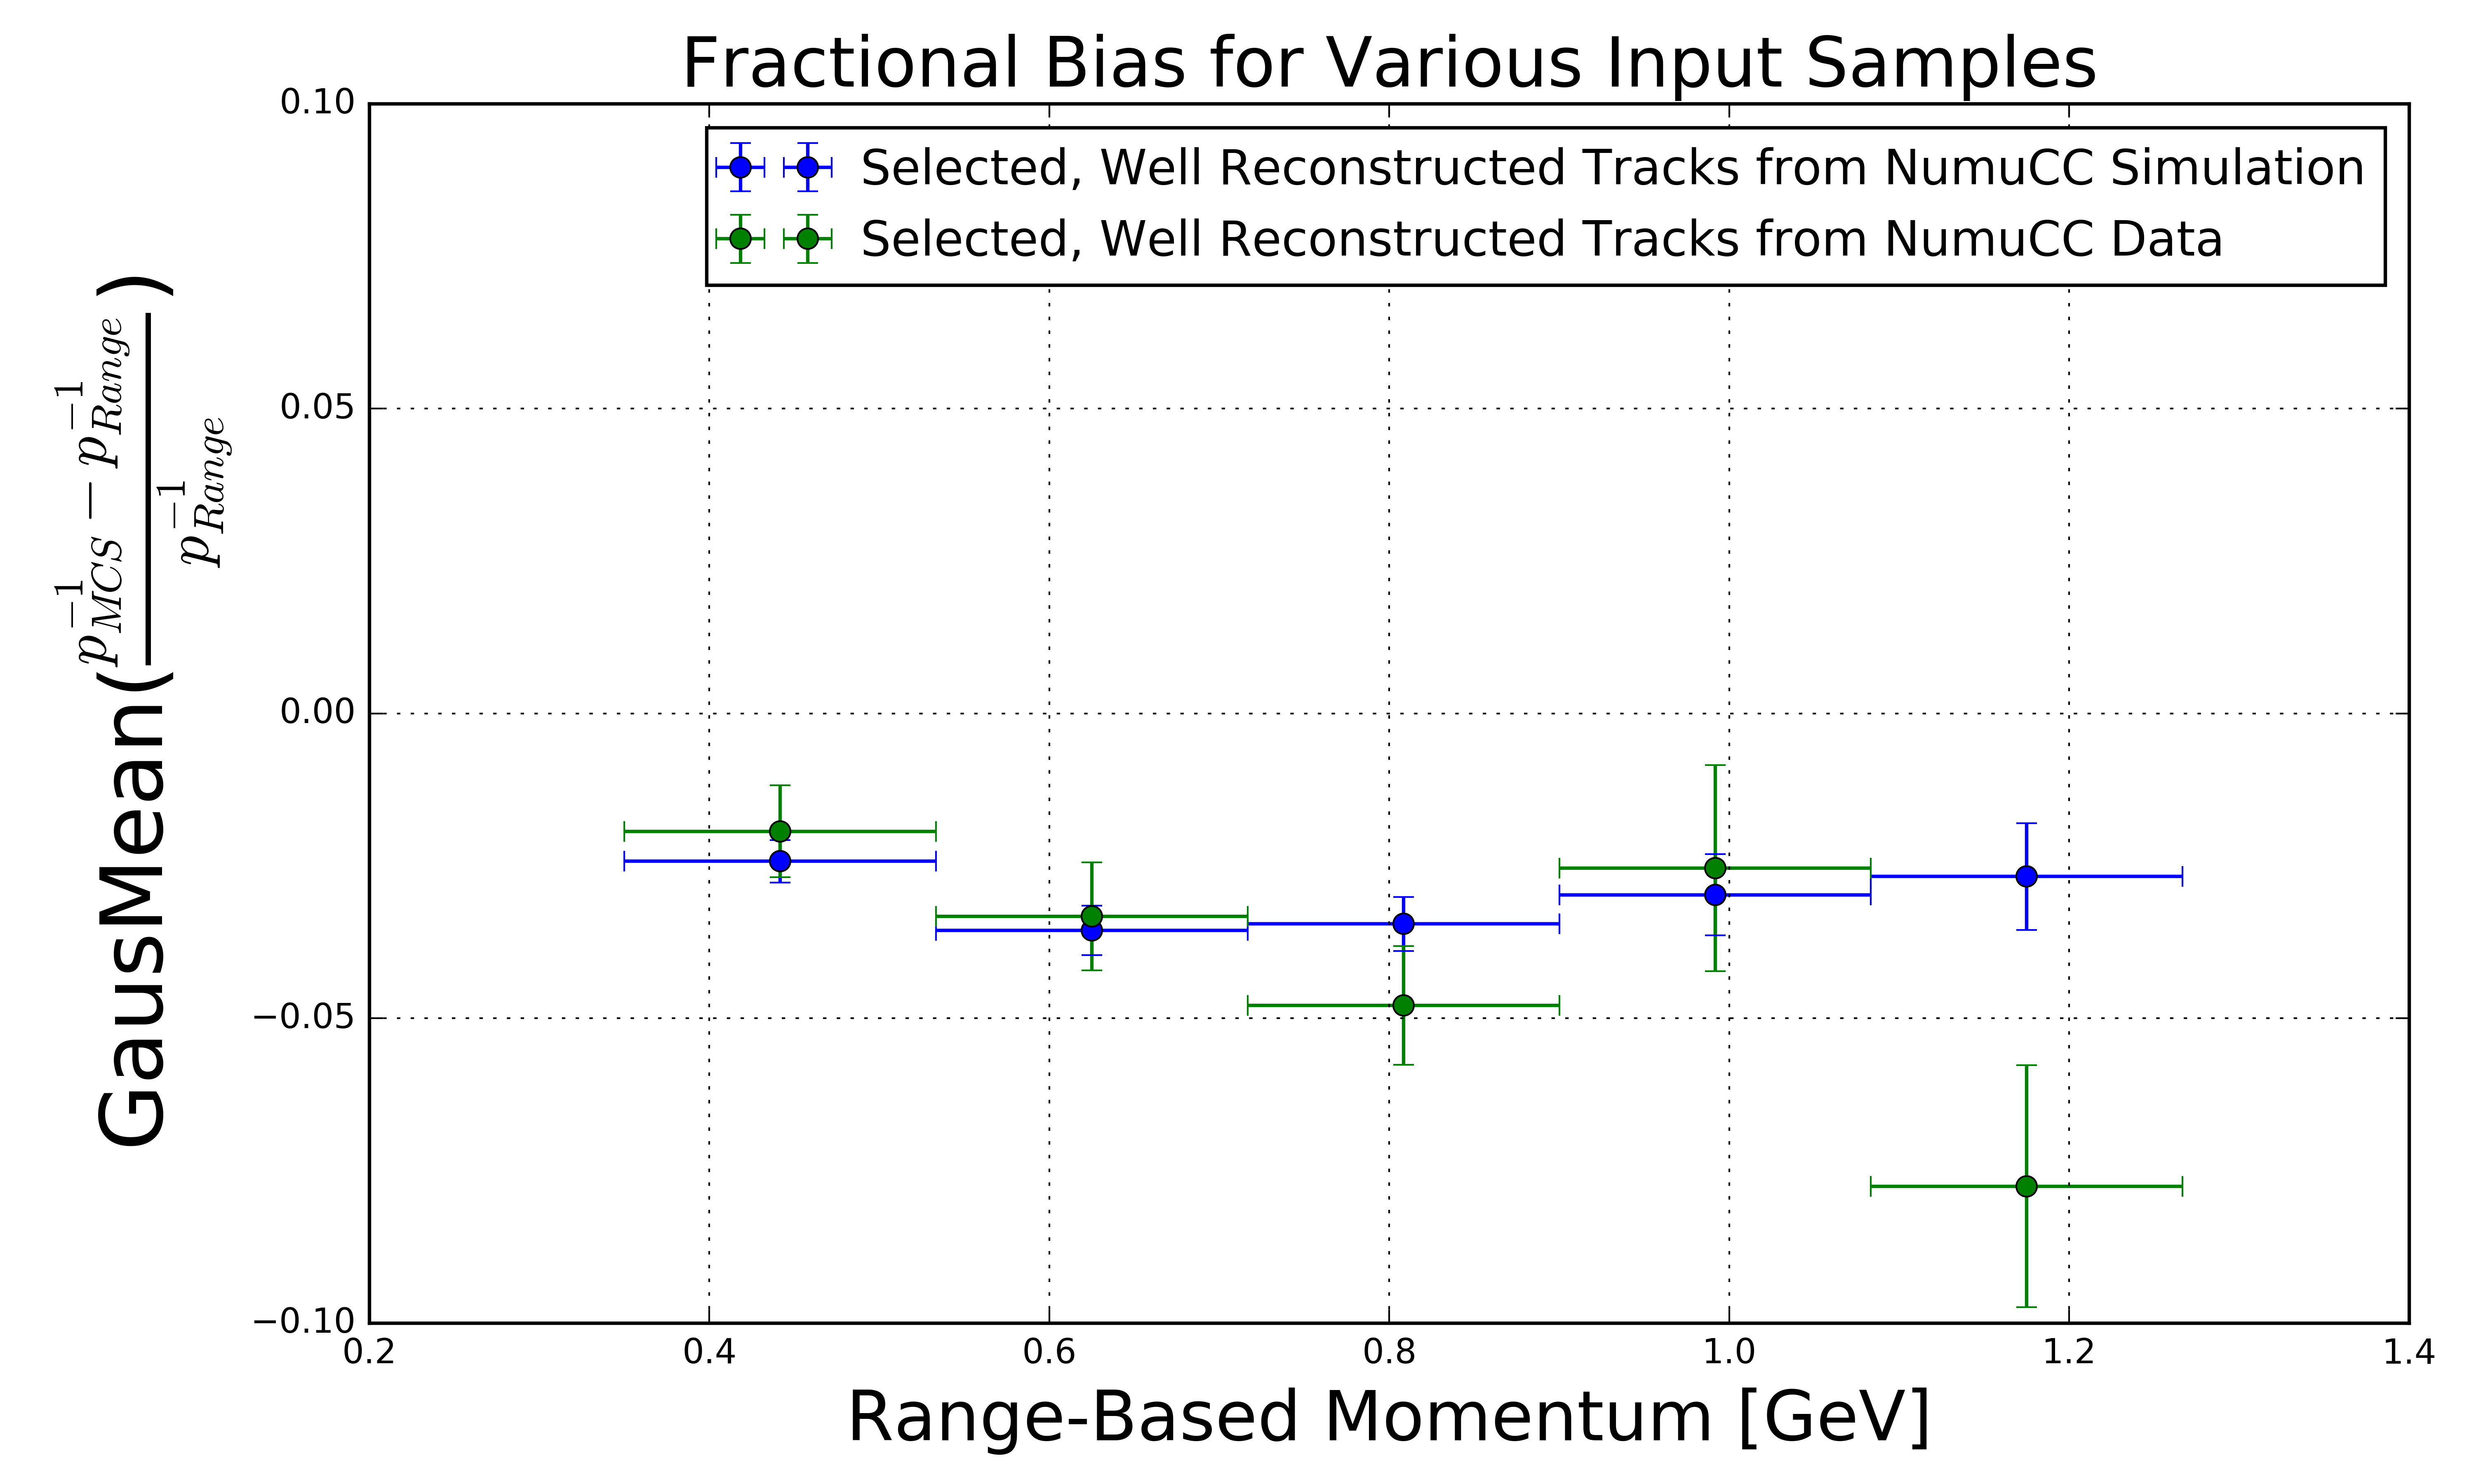
\includegraphics[width=0.9\textwidth]{Figures/MCS_range_bias_multiplesamples_publicplot.png}
	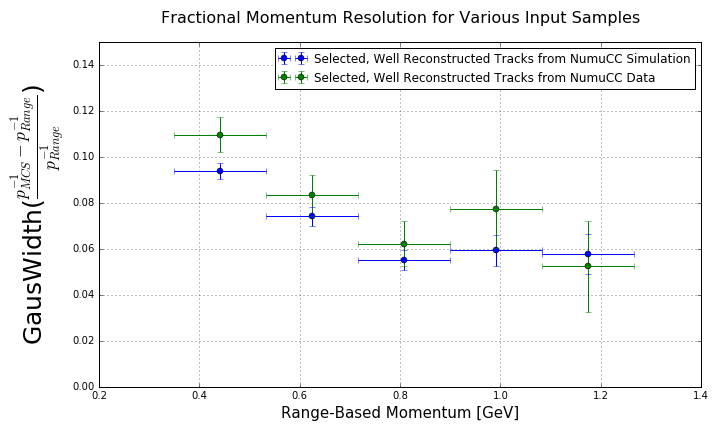
\includegraphics[width=0.9\textwidth]{Figures/MCS_range_resolution_multiplesamples_publicplot.png}
\caption{Inverse momentum difference (as defined in the text) fractional bias (top) and resolution (bottom) for automatically selected contained $\nu_\mu$CC-induced muons from full simulated BNB events with cosmic overlay where the track matches with the true muon track (blue), and automatically selected and hand-scanned (see text) contained $\nu_\mu$CC-induced muons from MicroBooNE data (green).}\label{MCS_range_bias_resolution_DataRecoTrack_fig}
\end{figure}

Figure \ref{MCS_range_bias_resolution_DataRecoTrack_fig} indicates a bias in the MCS momentum calculation on the order of a few percent, with a resolution that improves from about 10\% for contained reconstructed tracks in data and simulation with range momentum around 0.45 GeV/c (which corresponds to a length of about 1.5 m) to below 5\% for contained reconstructed tracks in data and simulation with range momentum about 1.15 GeV/c (which corresponds to a length of about 4.6 meters). Resolution improving with length of track is expected; the longer the track, the more angular scattering measurements can be made to improve the likelihood. In general the bias and resolutions agree between data and simulation within uncertainty.\\

\subsection{Impact of Highland formula tuning}\label{highland_formula_tuning_impact_section}

In order to examine the impact of the Highland formula tuning described in section \ref{highland_tuning_section}, the fractional bias and resolution on the simulated sample of contained muons described in section \ref{MCS_Momentum_Validation_DataRecoTrack_section} both with the nominal Highland formula (equation \ref{modified_highland_eqtn}) and with the retuned Highland formula (equation \ref{modified_highland_eqtn_kappa}) are shown in figure \ref{MCS_range_bias_resolution_compareHighlandFormulas_fig}. Tuning the Highland formula improves the magnitude of the fractional bias to below 2\%, and improves the fractional resolution by (2-3)\%, with the most improvement at the lowest momenta.

\begin{figure}
\centering
	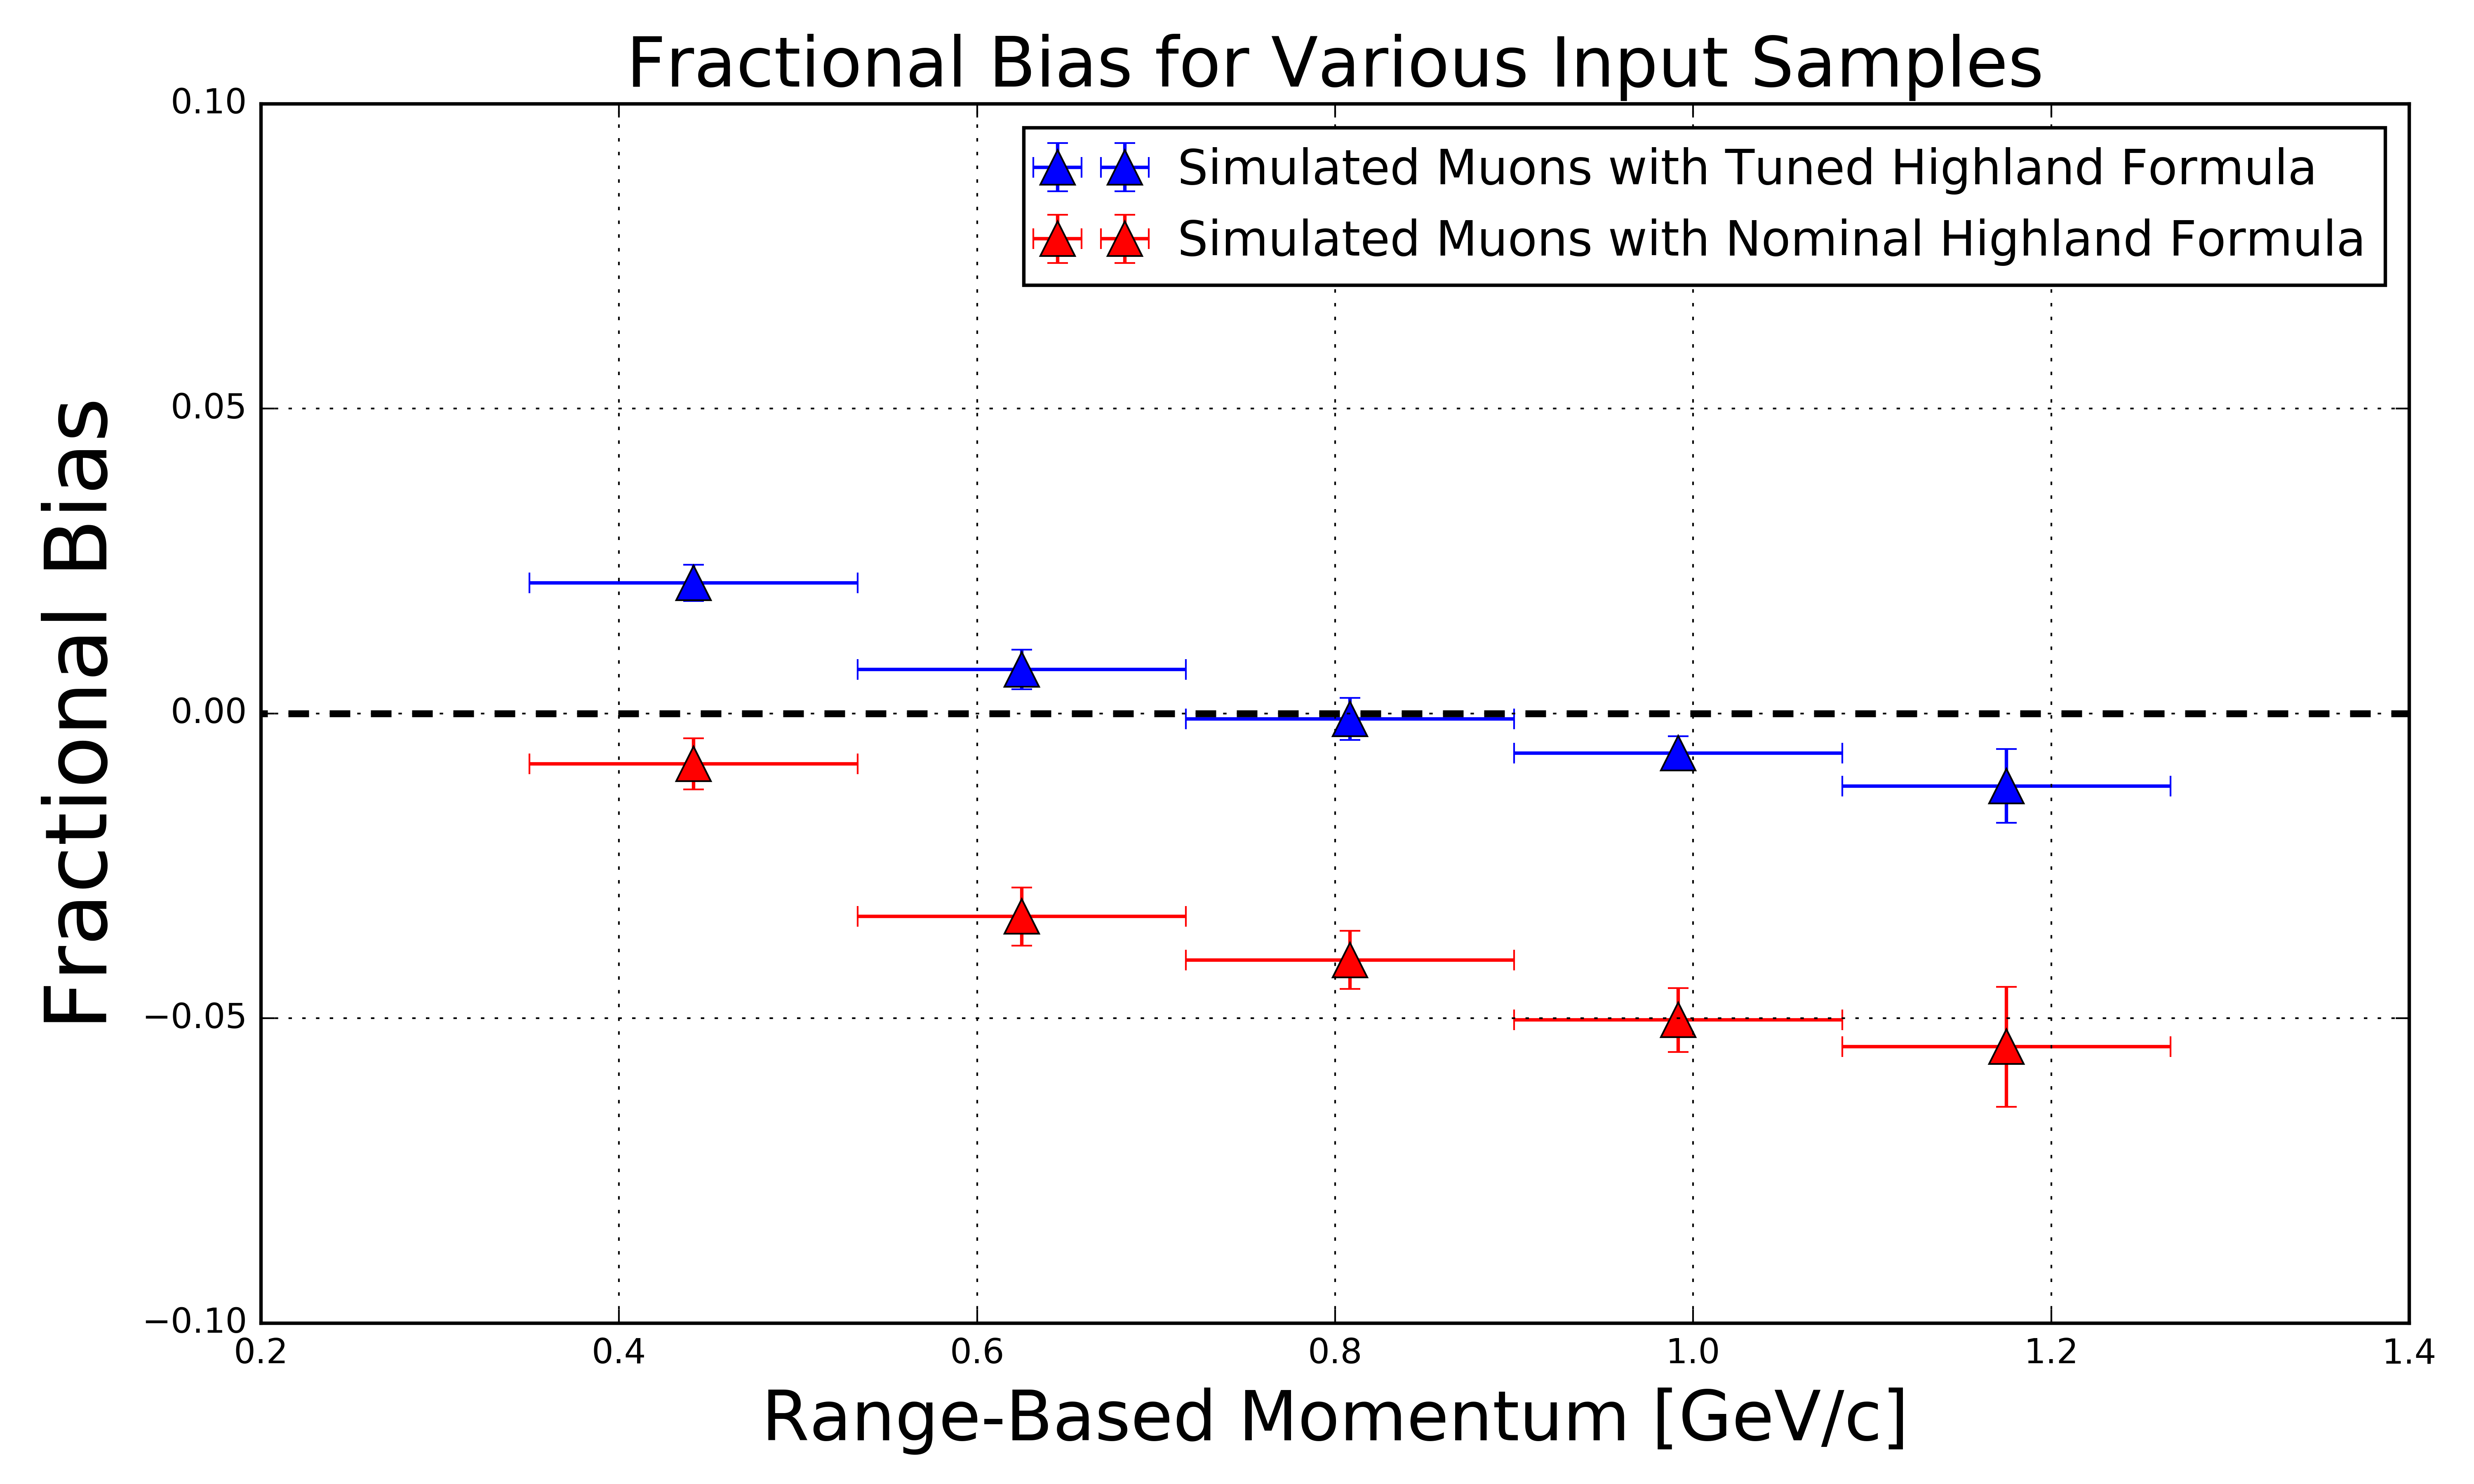
\includegraphics[width=0.9\textwidth]{Figures/MCS_range_bias_compareHighlandTuning_publicplot.png}
	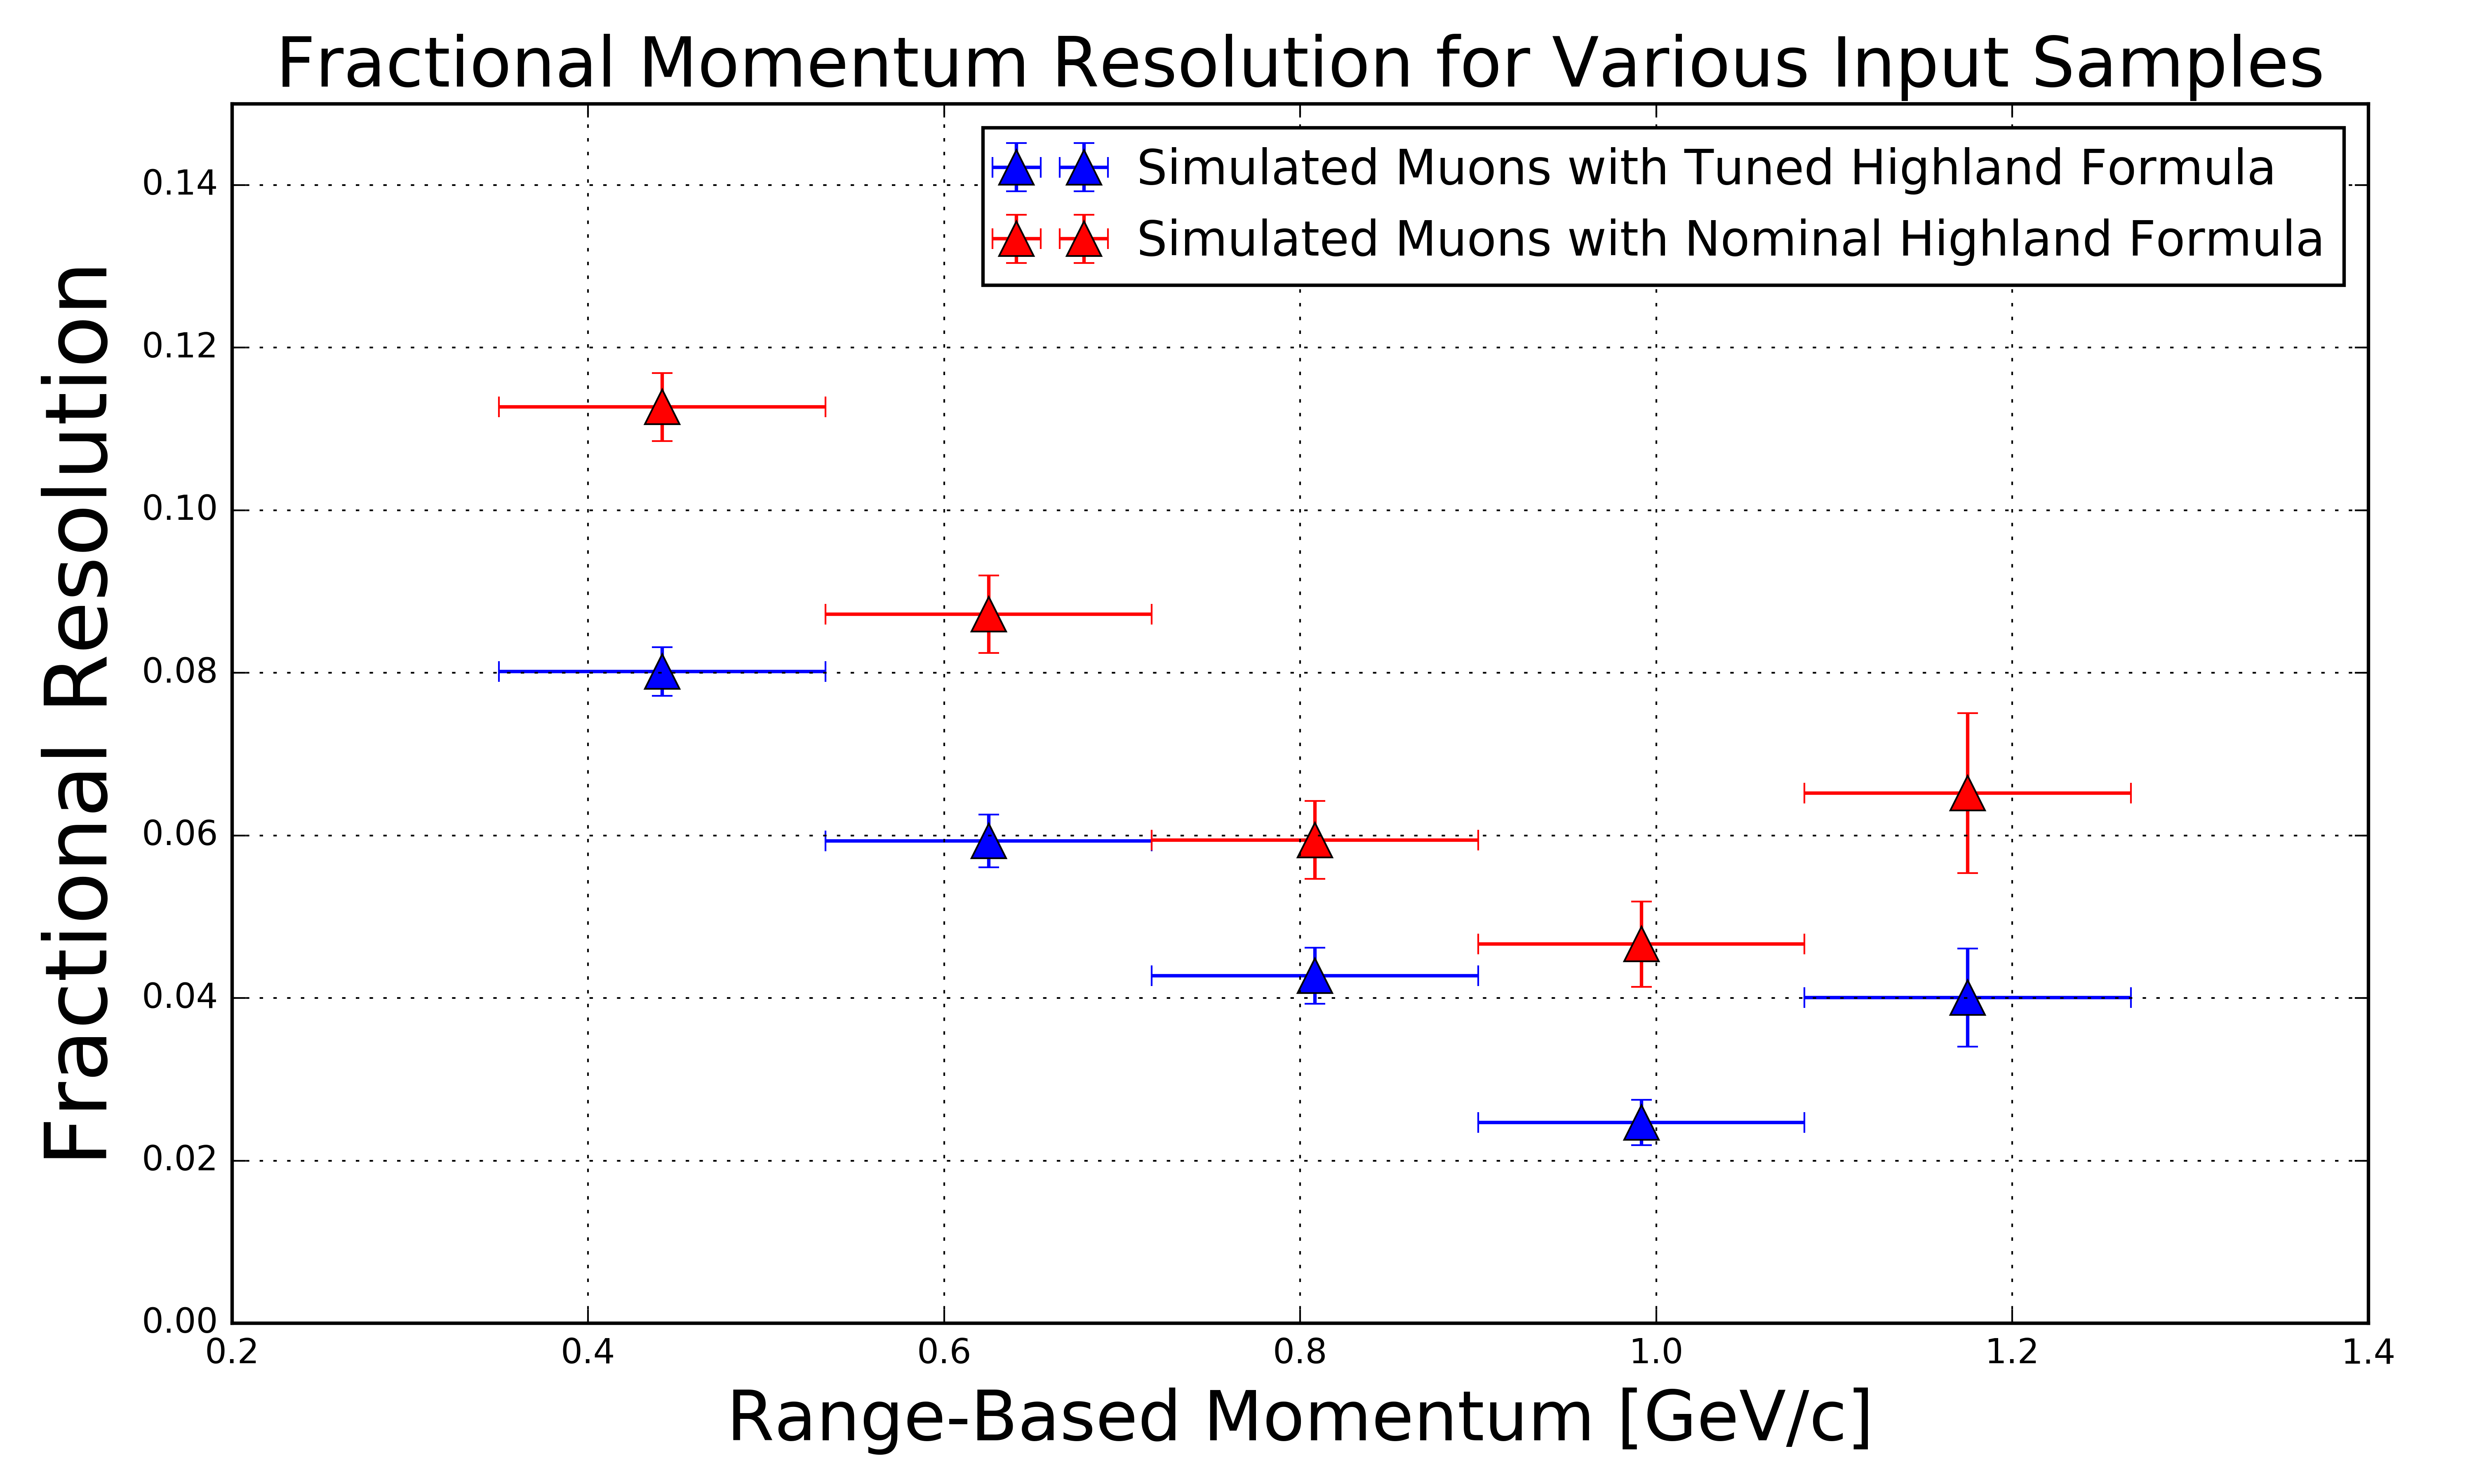
\includegraphics[width=0.9\textwidth]{Figures/MCS_range_resolution_compareHighlandTuning_publicplot.png}
\caption{Inverse momentum difference (as defined in the text) fractional bias (top) and resolution (bottom) for automatically selected contained $\nu_\mu$CC-induced muons from full simulated BNB events with cosmic overlay where the track matches with the true muon track both using the nominal Highland formula (equation \ref{modified_highland_eqtn}) (red) and the retuned Highland formula (equation \ref{modified_highland_eqtn_kappa}) (blue).}\label{MCS_range_bias_resolution_compareHighlandFormulas_fig}
\end{figure}






\section{MCS performance on exiting muons in MicroBooNE simulation}
In this section we quantify the MCS algorithm performance on a sample of well reconstructed exiting muon tracks in simulated BNB $\nu_\mu$CC interactions within the MicroBooNE detector. The tracks are automatically reconstructed by the same ``pandoraNuPMA'' algorithm described in section \ref{track_segmentation_and_scattering_angle_computation_section}, and all tracks have a length of at least $1$~m within the TPC. This simulation does not include space-charge effects. Approximately half of muons from $\nu_\mu$CC interactions within the specified fiducial volume exit the TPC, and about two thirds of those muons have at least one meter of track contained inside of the TPC. The relationship between the MCS and the true momenta at the beginning of the track as given by simulation for this sample of 28,000 exiting muon tracks is shown in figure \ref{MCS_true_comparison_exiting_fig}.\\

\begin{figure}[ht!]
\centering
	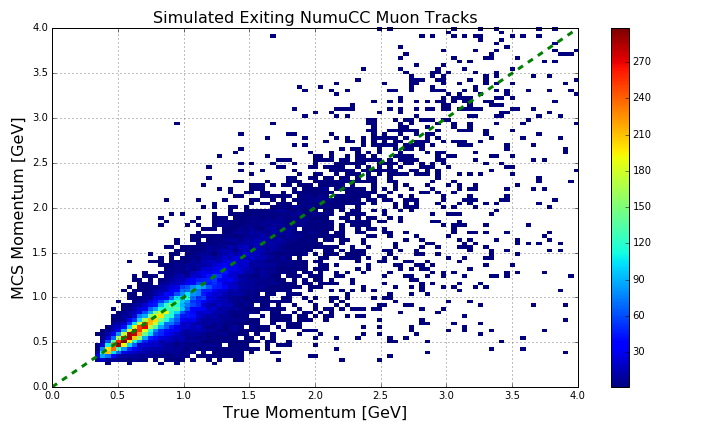
\includegraphics[width=0.9\textwidth]{Figures/MCS_true_comparison_MCBNBRecoTrackExiting.png} \\
\caption{MCS-computed momentum versus true momentum for the sample of simulated exiting BNB $\nu_\mu$CC muons in MicroBooNE with at least one meter of track contained within the TPC. The color (z) scale indicates number of tracks.}\label{MCS_true_comparison_exiting_fig}
\end{figure}

The distribution of $(p_{\text{MCS}}^{-1} - p_{\text{true}}^{-1})/(p_{\text{true}}^{-1})$ is shown for four representative bins of true momentum in figure \ref{MCS_true_exiting_resolution_MCBNBRecoTrackExiting_slices_fig}, along with the Gaussian fit to each distribution. Low-momentum tails where the MCS momentum is underestimated due to poor track reconstruction lie outside the fitted Gaussian function.\\

The fractional bias and resolution as a function of true momentum are shown in figure \ref{exitingRecoTrack_bias_resolution_fig_alllengths}. The bias is below 4\% for all momenta, and the resolution is $\approx$ 14\% in the relevant momentum region for BNB $\nu_\mu$CC muons (below 2 GeV/c). The resolution worsens for muon momenta above this region because the angular scatters begin to be comparable with the detector resolution term of 3 mrad. The resolution improves for longer lengths of track contained, with 10\% resolution for muons with $p<2$~$\text{GeV/c}$ with more than 3.5 meters contained. The mean length of track contained for muons in this analysis is 212 cm.\\


\begin{figure}
\centering
\includegraphics[width=0.45\textwidth]
	{Figures/{MCS_true_exiting_resolution_MCBNBRecoTrackExiting_slice_0.35_0.76}.png}
\includegraphics[width=0.45\textwidth]
	{Figures/{MCS_true_exiting_resolution_MCBNBRecoTrackExiting_slice_1.97_2.38}.png}
\includegraphics[width=0.45\textwidth]
	{Figures/{MCS_true_exiting_resolution_MCBNBRecoTrackExiting_slice_2.78_3.19}.png}
\includegraphics[width=0.45\textwidth]
	{Figures/{MCS_true_exiting_resolution_MCBNBRecoTrackExiting_slice_3.59_4.00}.png}
\caption{Fractional momentum difference for a few representative bins of true momentum for a sample of simulated exiting muon tracks. The y-axis is number of tracks, and the x-axis is $(p_{\text{MCS}}^{-1} - p_{\text{true}}^{-1})/(p_{\text{true}}^{-1})$.}
\label{MCS_true_exiting_resolution_MCBNBRecoTrackExiting_slices_fig}
\end{figure}

\begin{figure}
\centering
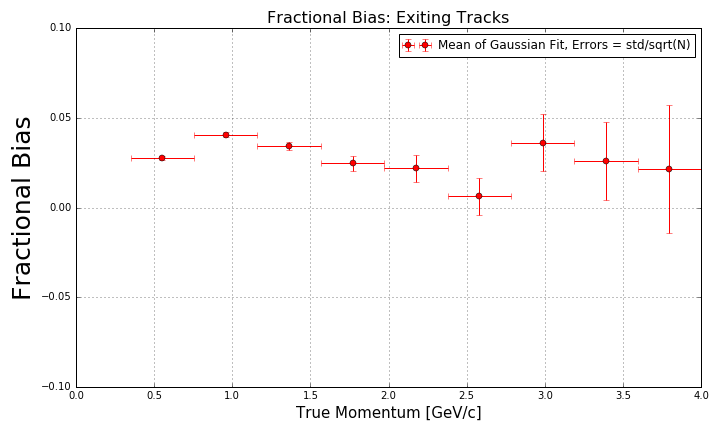
\includegraphics[width=0.9\textwidth]
	{Figures/MCS_true_exiting_bias_MCBNBRecoTrackExiting.png}
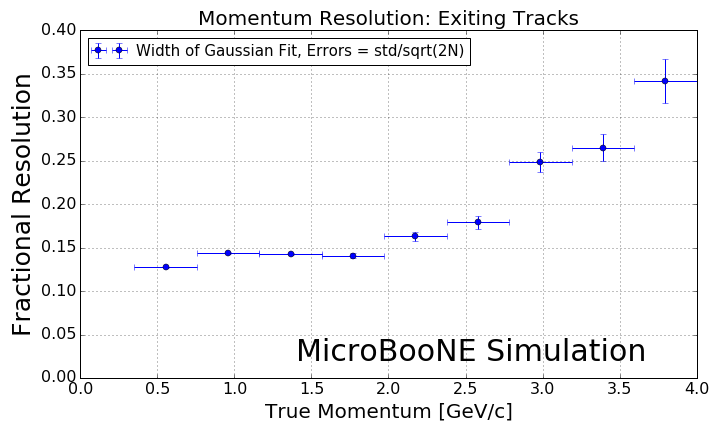
\includegraphics[width=0.9\textwidth]
	{Figures/MCS_true_exiting_resolution_MCBNBRecoTrackExiting.png}
\caption{MCS momentum fractional bias (top) and resolution (bottom) as a function of true momentum from a sample of exiting reconstructed muon tracks.}
\label{exitingRecoTrack_bias_resolution_fig_alllengths}
\end{figure}


% \begin{figure}
% \centering
% \mbox{
% 	\subfigure[\textit{MCS momentum bias. The vertical error bars are computed as $\frac{\sigma_{fit}}{\sqrt{N}}$, and the horizontal error bars indicate bin width.}\label{exitingRecoTrack_bias_fig_alllengths}]
% 	{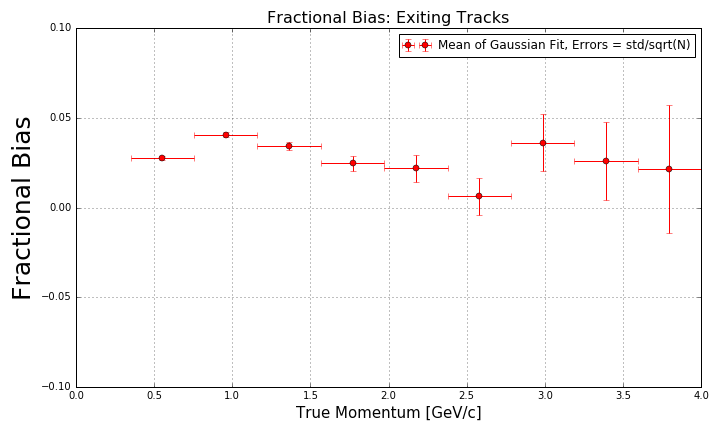
\includegraphics[width=75mm]{Figures/MCS_true_exiting_bias_MCBNBRecoTrackExiting.png}}
% 	\quad
% 	\subfigure[\textit{MCS momentum resolution. The vertical error bars are computed as $\frac{\sigma_{fit}}{\sqrt{2N}}$, and the horizontal error bars indicate bin width.}\label{exitingRecoTrack_resolution_fig_alllengths}]
% 	{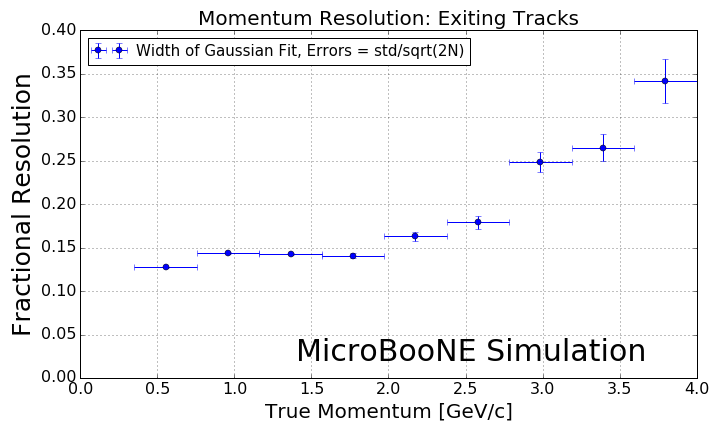
\includegraphics[width=75mm]{Figures/MCS_true_exiting_resolution_MCBNBRecoTrackExiting.png}}
% 	}
% \caption{\textit{MCS momentum bias as a function of true momentum for this sample of exiting muon reconstructed tracks. The vertical error bars are computed as $\frac{\sigma_{fit}}{\sqrt{N}}$, and the horizontal error bars indicate bin width.}}
% \end{figure}







\section{Conclusions}
We have described a multiple Coulomb scattering maximum likelihood method for estimating the momentum of a three dimensional reconstructed track in a LArTPC and have provided motivation for development of such a technique. Using simulation, we have shown that the standard Highland formula should be re-tuned specifically for scattering in liquid argon. After validating range-based momentum-determination techniques with MicroBooNE simulation, we have demonstrated the accuracy and precision of the MCS-based momentum reconstruction in MicroBooNE data by comparing its performance to the range-based method. For 398 fully-contained BNB $\nu_\mu$CC-induced muons, the MCS method exhibits a fractional bias below 3\% and a momentum resolution below 10\%, agreeing with simulation predictions. Using simulation of a separate sample of uncontained muon tracks in MicroBooNE with at least one meter contained in the active volume, the MCS-based reconstruction is shown to produce a fractional bias below 4\% and a momentum resolution of better than 15\% for muons in the relevant BNB energy region of below 2 GeV.

\acknowledgments
This material is based upon work supported by the following: the U.S. Department of Energy, Office of Science, Offices of High Energy Physics and Nuclear Physics; the U.S. National Science Foundation; the Swiss National Science Foundation; the Science and Technology Facilities Council of the United Kingdom; and The Royal Society (United Kingdom). Additional support for the laser calibration system and cosmic ray tagger was provided by the Albert Einstein Center for Fundamental Physics. Fermilab is operated by Fermi Research Alliance, LLC under Contract No. DE-AC02-07CH11359 with the United States Department of Energy.


% We suggest to always provide author, title and journal data:
% in short all the informations that clearly identify a document.
\clearpage
\begin{thebibliography}{99}

%These are sample bib items from the boilerplate template
% \bibitem{a}
% Author, \emph{Title}, \emph{J. Abbrev.} {\bf vol} (year) pg.

% \bibitem{b}
% Author, \emph{Title},
% arxiv:1234.5678.

% \bibitem{c}
% Author, \emph{Title},
% Publisher (year).

%1
  \bibitem{Aguilar-Arevalo:2013pmq} 
  A.~A.~Aguilar-Arevalo {\it et al.} 
  [MiniBooNE Collaboration],
  \textit{Improved Search for $\bar \nu_\mu \rightarrow \bar \nu_e$ Oscillations in the MiniBooNE Experiment},
  Phys.\ Rev.\ Lett.\  {\bf 110}, 161801 (2013).

  [arXiv:1207.4809 [hep-ex], arXiv:1303.2588 [hep-ex]].

  %384 citations counted in    

\bibitem{SBNwhitepaper} 
  C.~Adams {\it et al.} [LArTPC Collaboration],
  \textit{LAr1-ND: Testing Neutrino Anomalies with Multiple LArTPC Detectors at Fermilab},
  arXiv:1309.7987 [physics.ins-det].
  %%CITATION = ARXIV:1309.7987;%%
  %28 citations counted in INSPIRE as of 03 Feb 2017

 \bibitem{ICARUS_maincitation}
  F.~Arneodo {\it et al.} [ICARUS Collaboration],
  \textit{The ICARUS experiment: A Second generation proton decay experiment and neutrino observatory at the Gran Sasso Laboratory},
  hep-ex/0103008.
  %%CITATION = HEP-EX/0103008;%%
  %73 citations counted in INSPIRE as of 13 Feb 2017

  \bibitem{DUNE_citation}
  R.~Acciarri {\it et al.} [DUNE Collaboration],
  \textit{Long-Baseline Neutrino Facility (LBNF) and Deep Underground Neutrino Experiment (DUNE) : Volume 1: The LBNF and DUNE Projects},
  arXiv:1601.05471 [physics.ins-det].
  %%CITATION = ARXIV:1601.05471;%%
  %56 citations counted in INSPIRE as of 13 Feb 2017

  \bibitem{ub_detectorpaper} 
  R.~Acciarri {\it et al.} [MicroBooNE Collaboration],
  \textit{Design and Construction of the MicroBooNE Detector},
  arXiv:1612.05824 [physics.ins-det].
  %%CITATION = ARXIV:1612.05824;%%

  \bibitem{BNB_citation}
  A.~A.~Aguilar-Arevalo {\it et al.} [MiniBooNE Collaboration],
  \textit{The Neutrino Flux prediction at MiniBooNE},
  Phys.\ Rev.\ D {\bf 79}, 072002 (2009)

  [arXiv:0806.1449 [hep-ex]].

  %224 citations counted in INSPIRE as of 13 Feb 2017

  % \bibitem{SCE_publicnote}
  % R.~Acciarri {\it et al.} [MicroBooNE Collaboration],
  % \textit{Study of Space Charge Effects in MicroBooNE},
  % www-microboone.fnal.gov/publications/publicnotes/MICROBOONE-NOTE-1018-PUB.pdf.

  % %2
  % \bibitem{lartpc}
  % S. ~Lockwitz, 
  % The MicroBooNE LArTPC,
  % http://www-microboone.fnal.gov/talks/dpfMicroBooNELArTPC.pdf.

  %4
  \bibitem{highland}
  V. ~L. ~Highland, 
  \textit{Some Practical Remarks on Multiple Scattering},
  Nucl.\ Instrum.\ Methods\ {\bf 129} (1975)
  104-120.
 
   \bibitem{highland-lynch-dahl}
  G. R. Lynch and O. I. Dahl, Nucl.\ Instrum.\ Methods\, 
  Section B (Beam Interactions with Materials and Atoms) {\bf B58, 6} (1991). 

 \bibitem{DONUT_paper} 
  K.~Kodama {\it et al.} [DONUT Collaboration],
  \textit{Observation of tau neutrino interactions},
  Phys.\ Lett.\ B {\bf 504}, 218 (2001)

  [hep-ex/0012035].

    \bibitem{OPERA_paper}
  N.~Agafonova {\it et al.} [OPERA Collaboration],
  \textit{Momentum measurement by the Multiple Coulomb Scattering method in the OPERA lead emulsion target},
  New J.\ Phys.\  {\bf 14}, 013026 (2012)
  [arXiv:1106.6211 [physics.ins-det]].

 
  \bibitem{MACRO_paper} 
  G.~Giacomelli [MACRO Collaboration],
  \textit{Neutrino physics and astrophysics with the MACRO experiment at the Gran Sasso lab},
  Braz.\ J.\ Phys.\  {\bf 33}, 211 (2003)

  [hep-ex/0210006].

  \bibitem{icarus_mcs_paper}
  A.~Ankowski {\it et al.} [ICARUS Collaboration],
  \textit{Measurement of through-going particle momentum by means of multiple scattering with the ICARUS T600 TPC},
  Eur.\ Phys.\ J.\ C {\bf 48}, 667 (2006)
  [hep-ex/0606006].

  %44 citations counted in INSPIRE as of 01 Dec 2016

  \bibitem{new_icarus_paper}
  M.~Antonello {\it et al.},
  \textit{Muon momentum measurement in ICARUS-T600 LAr-TPC via multiple scattering in few-GeV range},
  arXiv:1612.07715 [physics.ins-det].


  \bibitem{GEANT4_citation}
  S. Agostinelliet al. Nucl.\ Instrum.\ Methods Phys.\ Res.\ {\bf A506250-303} (2003)


  \bibitem{LARIAT_citation} 
  F.~Cavanna {\it et al.} [LArIAT Collaboration],
  \textit{LArIAT: Liquid Argon In A Testbeam},
  arXiv:1406.5560 [physics.ins-det].
  %%CITATION = ARXIV:1406.5560;%%
  %18 citations counted in INSPIRE as of 03 Feb 2017

  %%CITATION = ARXIV:1612.07715;%%
  % %5
  % \bibitem{leonidas1}
  % L. ~Kalousis, 
  % Momentum measurement via Multiple Coulomb
  % Scattering with the MicroBooNE detector, 
  % MicroBooNE Doc-DB-3733.


  % %3
  % \bibitem{leonidas2}
  % L. ~Kalousis, 
  % Muon momentum measurement via Multiple Coulomb Scattering in argon,
  % MicroBooNE Doc-DB-4050.

 %7
  \bibitem{Marshall:2015rfa} 
  J.~S.~Marshall and M.~A.~Thomson,
  \textit{The Pandora Software Development Kit for Pattern Recognition},
  Eur.\ Phys.\ J.\ C {\bf 75}, no. 9, 439 (2015)

  [arXiv:1506.05348 [physics.data-an]].

  %8
  \bibitem{MIPenergysource}
  D. E. Groom, N. V. Mokhov and S. Striganov,
  \textit{Muon Stopping Power and Range Tables: 10 MeV - 100 TeV} Table 5,
  http://pdg.lbl.gov/2012/AtomicNuclearProperties/adndt.pdf

  \bibitem{stoppingpowersource}
  H. Bichsel, D. E. Groom, S.R. Klein, 
  \textit{Passage of Particles Through Matter} PDG Chapter 27, Figure 27.1 \url{http://pdg.lbl.gov/2005/reviews/passagerpp.pdf}

  %9`'
  \bibitem{PDG_spline_table} Table 289: Muons in Liquid argon (Ar) \url{http://pdg.lbl.gov/2012/AtomicNuclearProperties/MUON_ELOSS_TABLES/muonloss_289.pdf}

  \bibitem{NISTdata} \textit{Stopping Powers and Ranges for Protons and Alpha Particles}, ICRU Report No. 49 (1993); Tables and graphs of these data are available at \url{http://physics.nist.gov/PhysRefData/}

  \bibitem{corsika_ref} D. Heck, J. Knapp, J. N. Capdevielle, G. Schatz, T. Throw, \textit{CORSIKA: A Monte Carlo Code to Simulate Extensive Air Showers}, Forschungszentrum Karlsruhe Report FZKA 6019 (1998)

  % %6
  % \bibitem{CCIncInternalNote}
  % An et al,
  % Selection of charged-current $\nu_\mu$ inclusive events - Internal Note,
  % MicroBooNE Doc-DB-5851
  % \url{http://microboone-docdb.fnal.gov:8080/cgi-bin/RetrieveFile?docid=5851&filename=cc-incl-neutrino2016-v2.7.pdf&version=9}





% Please avoid comments such as "For a review'', "For some examples",
% "and references therein" or move them in the text. In general,
% please leave only references in the bibliography and move all
% accessory text in footnotes.

% Also, please have only one work for each \bibitem.


\end{thebibliography}
\end{document}




%%%%%%%%%%%%%%%%%%% ORIGINAL JINST BOILERPLATE CONTENT BELOW %%%%%%%%%%%%%%%%%%%%%%%%%%%%%%%
% For internal references use label-refs: see section~\ref{sec:intro}.
% Bibliographic citations can be done with cite: refs.~\cite{a,b,c}.
% When possible, align equations on the equal sign. The package
% \texttt{amsmath} is already loaded. See \eqref{eq:x}.
% \begin{equation}
% \label{eq:x}
% \begin{split}
% x &= 1 \,,
% \qquad
% y = 2 \,,
% \\
% z &= 3 \,.
% \end{split}
% \end{equation}
% Also, watch out for the punctuation at the end of the equations.


% If you want some equations without the tag (number), please use the available
% starred-environments. For example:
% \begin{equation*}
% x = 1
% \end{equation*}

% The amsmath package has many features. For example, you can use use
% \texttt{subequations} environment:
% \begin{subequations}\label{eq:y}
% \begin{align}
% \label{eq:y:1}
% a & = 1
% \\
% \label{eq:y:2}
% b & = 2
% \end{align}
% and it will continue to operate across the text also.
% \begin{equation}
% \label{eq:y:3}
% c = 3
% \end{equation}
% \end{subequations}
% The references will work as you'd expect: \eqref{eq:y:1},
% \eqref{eq:y:2} and \eqref{eq:y:3} are all part of \eqref{eq:y}.

% A similar solution is available for figures via the \texttt{subfigure}
% package (not loaded by default and not shown here).
% All figures and tables should be referenced in the text and should be
% placed on the page where they are first cited or in
% subsequent pages. Positioning them in the source file
% after the paragraph where you first reference them usually yield good
% results. See figure~\ref{fig:i} and table~\ref{tab:i}.

% \begin{figure}[htbp]
% \centering % \begin{center}/\end{center} takes some additional vertical space
% \includegraphics[width=.4\textwidth,trim=30 110 0 0,clip]{example-image-a}
% \qquad
% \includegraphics[width=.4\textwidth,origin=c,angle=180]{example-image-b}
% % "\includegraphics" from the "graphicx" permits to crop (trim+clip)
% % and rotate (angle) and image (and much more)
% \caption{\label{fig:i} Always give a caption.}
% \end{figure}


% \begin{table}[htbp]
% \centering
% \caption{\label{tab:i} We prefer to have borders around the tables.}
% \smallskip
% \begin{tabular}{|lr|c|}
% \hline
% x&y&x and y\\
% \hline
% a & b & a and b\\
% 1 & 2 & 1 and 2\\
% $\alpha$ & $\beta$ & $\alpha$ and $\beta$\\
% \hline
% \end{tabular}
% \end{table}

% We discourage the use of inline figures (wrapfigure), as they may be
% difficult to position if the page layout changes.

% We suggest not to abbreviate: ``section'', ``appendix'', ``figure''
% and ``table'', but ``eq.'' and ``ref.'' are welcome. Also, please do
% not use \texttt{\textbackslash emph} or \texttt{\textbackslash it} for
% latin abbreviaitons: i.e., et al., e.g., vs., etc.



% \section{Sections}
% \subsection{And subsequent}
% \subsubsection{Sub-sections}
% \paragraph{Up to paragraphs.} We find that having more levels usually
% reduces the clarity of the article. Also, we strongly discourage the
% use of non-numbered sections (e.g.~\texttt{\textbackslash
%   subsubsection*}).  Please also see the use of
% ``\texttt{\textbackslash texorpdfstring\{\}\{\}}'' to avoid warnings
% from the hyperref package when you have math in the section titles



% \appendix
% \section{Some title}
% Please always give a title also for appendices.





% \acknowledgments

% This is the most common positions for acknowledgments. A macro is
% available to maintain the same layout and spelling of the heading.

% \paragraph{Note added.} This is also a good position for notes added
% after the paper has been written.





